\documentclass[10pt]{beamer}
\usetheme{Boadilla} % My favorite!
\setbeamercovered{invisible}
% To remove the navigation symbols from
% the bottom of slides%
\setbeamertemplate{navigation symbols}{}
\setbeamertemplate{itemize items}[default]
\setbeamertemplate{enumerate items}[default]
\xdefinecolor{lavendar}{rgb}{0.2, 0.2, 0.72}
%
\usepackage{graphicx,epsfig}
\usepackage{tikz}
\usetikzlibrary{mindmap,trees,shadows,backgrounds}

%\usepackage{bm}         % For typesetting bold math (not \mathbold)
%\logo{\includegraphics[height=0.6cm]{yourlogo.eps}}
%
\newcommand{\be}{\begin{equation*}}
\newcommand{\ee}{\end{equation*}}
\newcommand{\ba}{\begin{eqnarray}}
\newcommand{\ea}{\end{eqnarray}}

\newcommand{\vso}{\vskip15pt}
\newcommand{\vst}{\vskip30pt}
\newcommand{\nsub}{n_\mathrm{sub}}

\def\smallfrac#1#2{\hbox{${{#1}\over {#2}}$}}

\title[]{Parton distributions with LHC data}
\author{Nathan Hartland}
\institute
{
University of Edinburgh\\
%
\includegraphics[height=2cm]{edinburghcrest.pdf}
\medskip
}
% \today will show current date.
% Alternatively, you can specify a date.
%

\date{\today}


\begin{document}
\renewcommand{\inserttotalframenumber}{18}


\begin{frame}
\begin{centering}
\vskip20pt
\center{\huge\color{lavendar} \textbf{Update on NNPDF parton distributions}}
\vskip20pt
Nathan Hartland\\

\small{The University of Edinburgh}\\
\vso

\begin{center} \hskip10pt 
\includegraphics[height=1cm]{nnpdf_logo_official.eps} \end{center}


\vskip10pt
{\bf The NNPDF Collaboration:}\\
R.~D.~Ball, V.~Bertone, S.~Carrazza,\\ F.~Cerutti,
C.~Deans, L.~Del~Debbio, S~Forte,\\
A~Guffanti, N.H, J.I.~Latorre, J.~Rojo and M.~Ubiali.
\vskip20pt
DIS 2013, Marseille\\
Tuesday 23nd April 2013

\end{centering}

\end{frame}



\begin{frame}
\frametitle{Current status of NNPDF determinations}

\begin{itemize}
 \item<1->{  \small Most recent update: \textbf{NNPDF2.3} includes constraints from LHC data}\vskip10pt
 \end{itemize}

\begin{columns}
  \begin{column}{0.4\textwidth}  \vskip-20pt
  \underline{New data in 2.3}
  \vskip2pt
\begin{itemize}
\item<1->{ \small \textbf{ATLAS 2010} \\Inclusive Jets, \\W$^{\pm}$/Z rapidity distributions. }
\item<1->{ \small \textbf{LHCb 2010} \\W$^{\pm}$ rapidity distributions. }
\item<1->{ \small \textbf{CMS  2011} \\W lepton asymmetry.}
\end{itemize}
   \end{column}

 % \hskip-35pt
   \begin{column}{0.6\textwidth}
      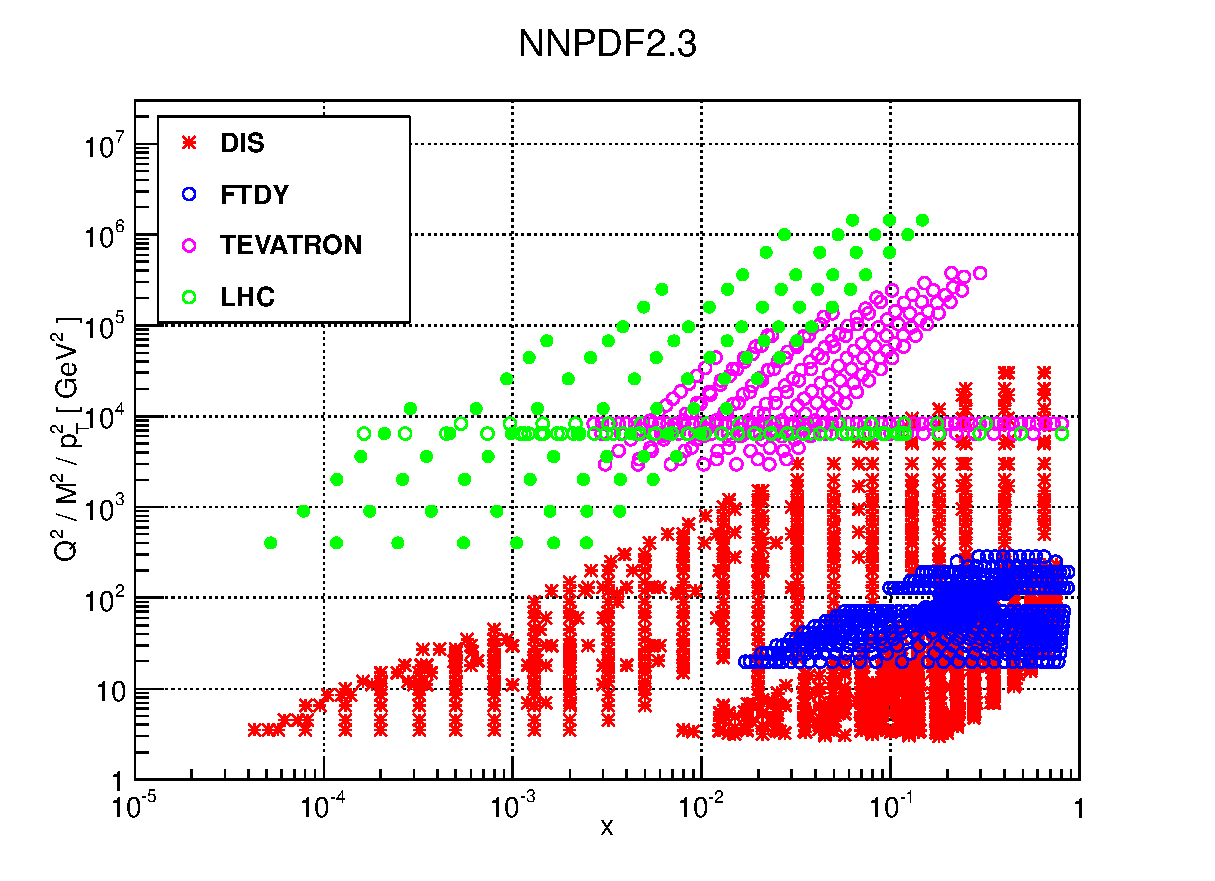
\includegraphics[width=1.0\textwidth]{kin23}

   \end{column}
\end{columns}

\small{
\underline{NNPDF2.3 Family}\\
\vskip5pt
\textbf{NNPDF2.3} - global dataset including LHC data.\\
\textbf{NNPDF2.3 noLHC} - global dataset without LHC data.\\
\textbf{NNPDF2.3 Collider} - HERA, Tevatron and LHC data only.\\}

\end{frame}

\begin{frame}
\frametitle{Constraints from LHC data}
\begin{center}
   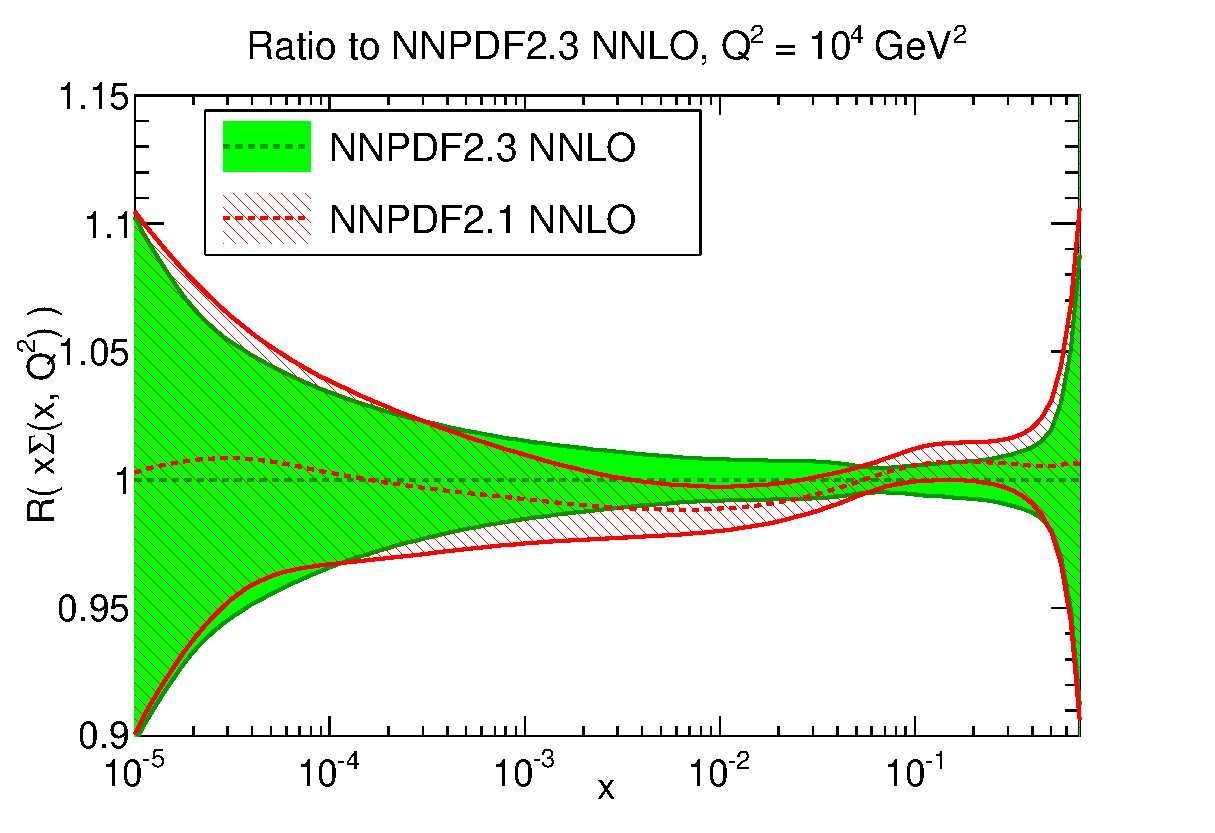
\includegraphics[width=0.4\textwidth]{xSinglet_Q_10000_log-rat-21-vs-23-nnlo.eps}
 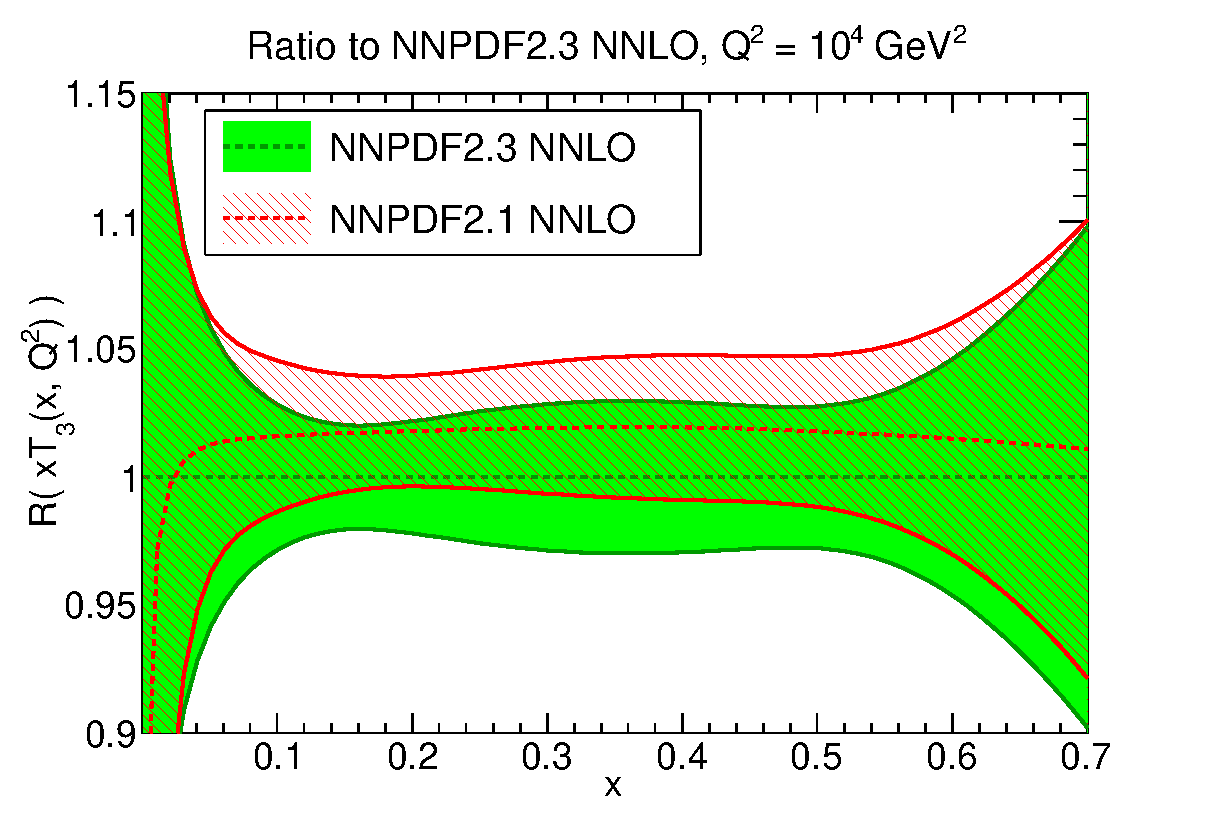
\includegraphics[width=0.4\textwidth]{xT3_Q_10000_lin-rat-21-vs-23-nnlo.eps}\\
     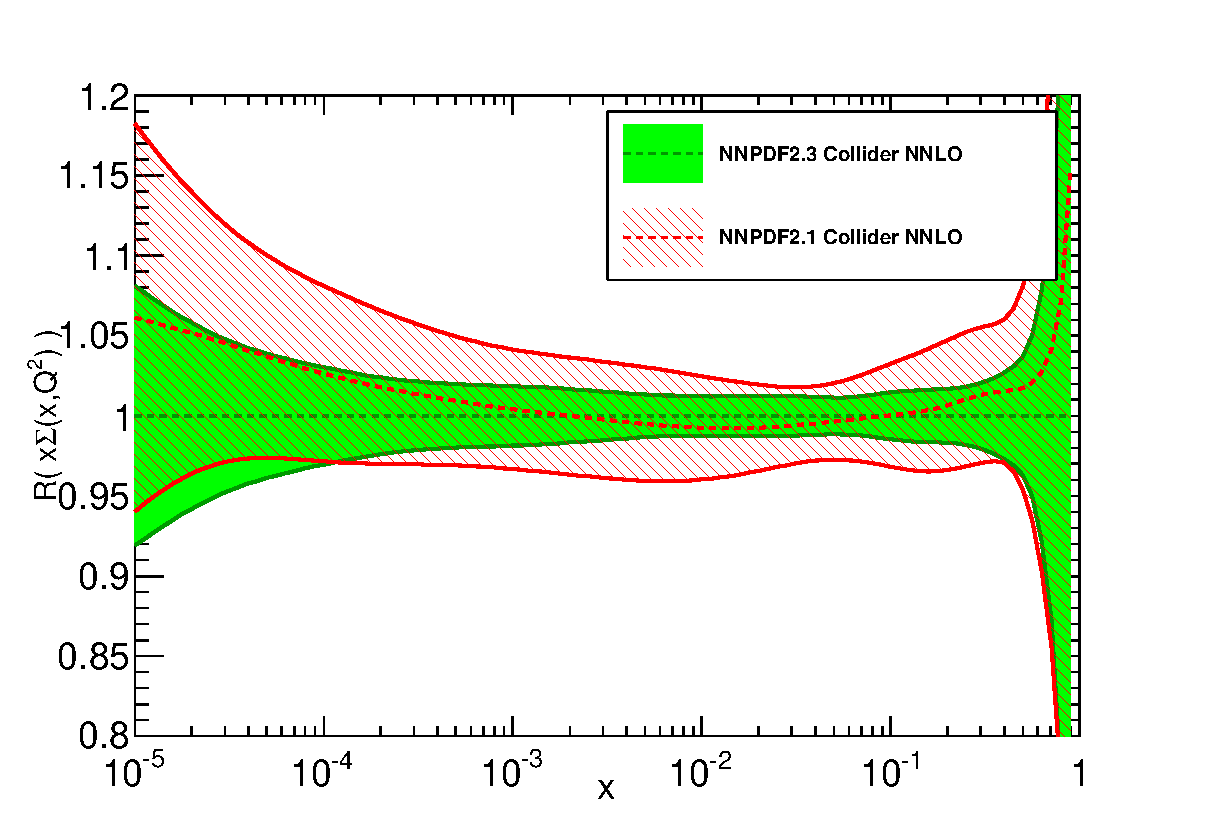
\includegraphics[width=0.4\textwidth]{colliderSigma.eps}
 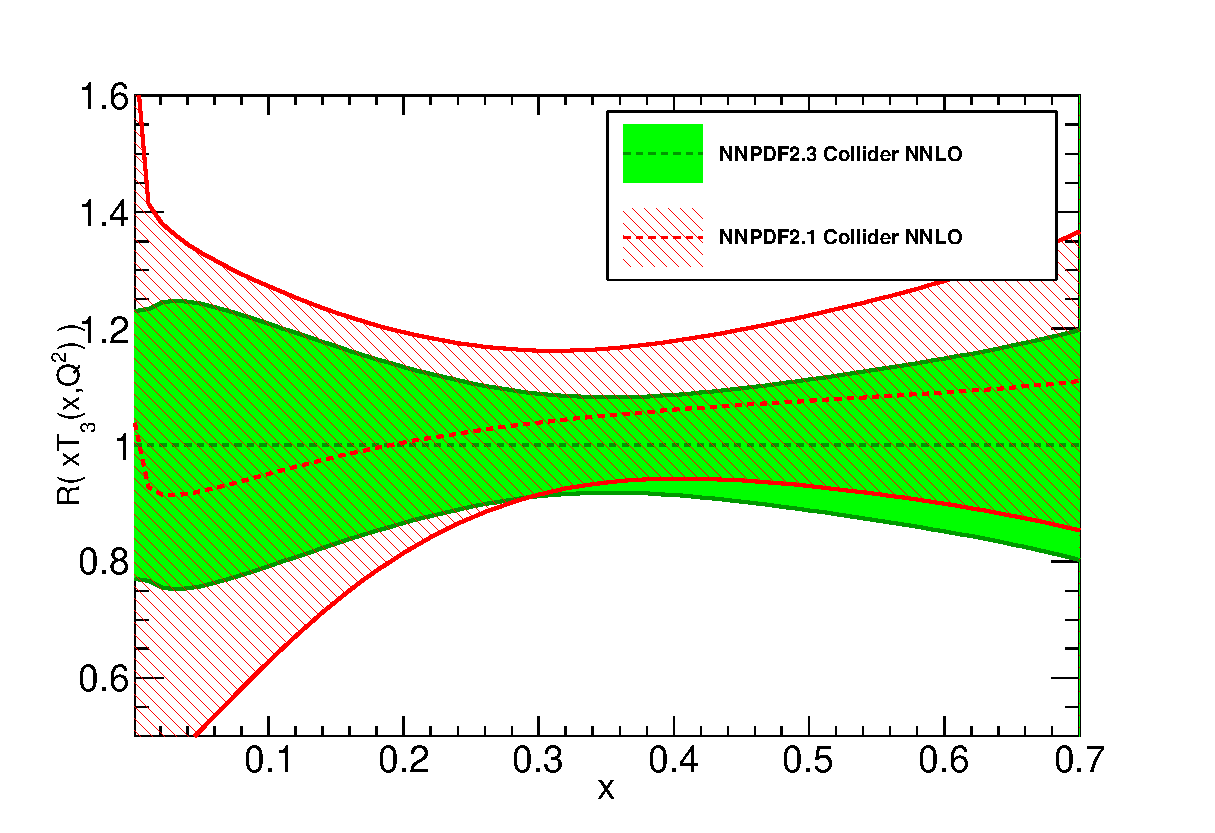
\includegraphics[width=0.4\textwidth]{colliderT3.eps}
 \end{center}
 \begin{itemize}
 \item<1-> LHC data generally demonstrates good consistency with the global dataset.
  \item<1-> Provides particularly large constraint for collider only PDFs.

 \end{itemize}
 \end{frame}


\begin{frame}
\frametitle{The strange content of the proton.}

Strange distributions suffer from generally large uncertainties.

   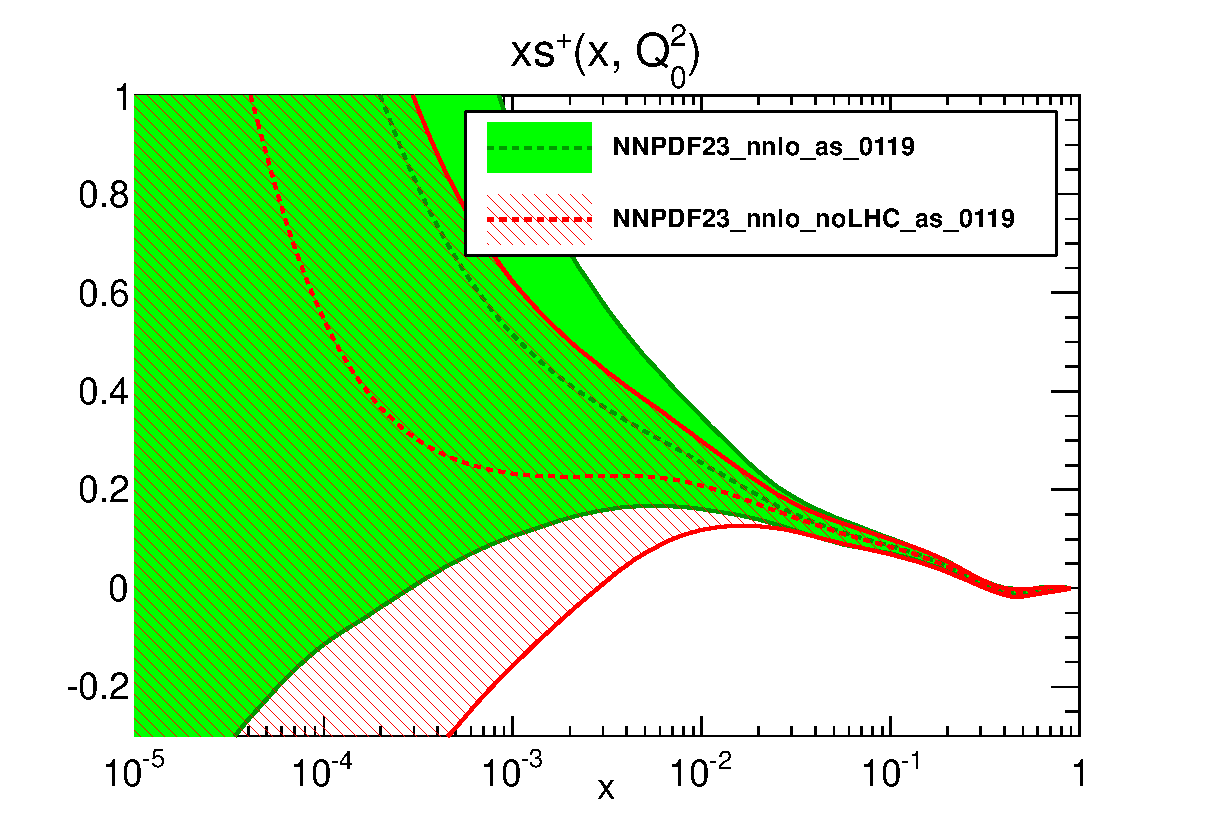
\includegraphics[width=0.5\textwidth]{pdf_xsplus_log_band_comparison.eps}
   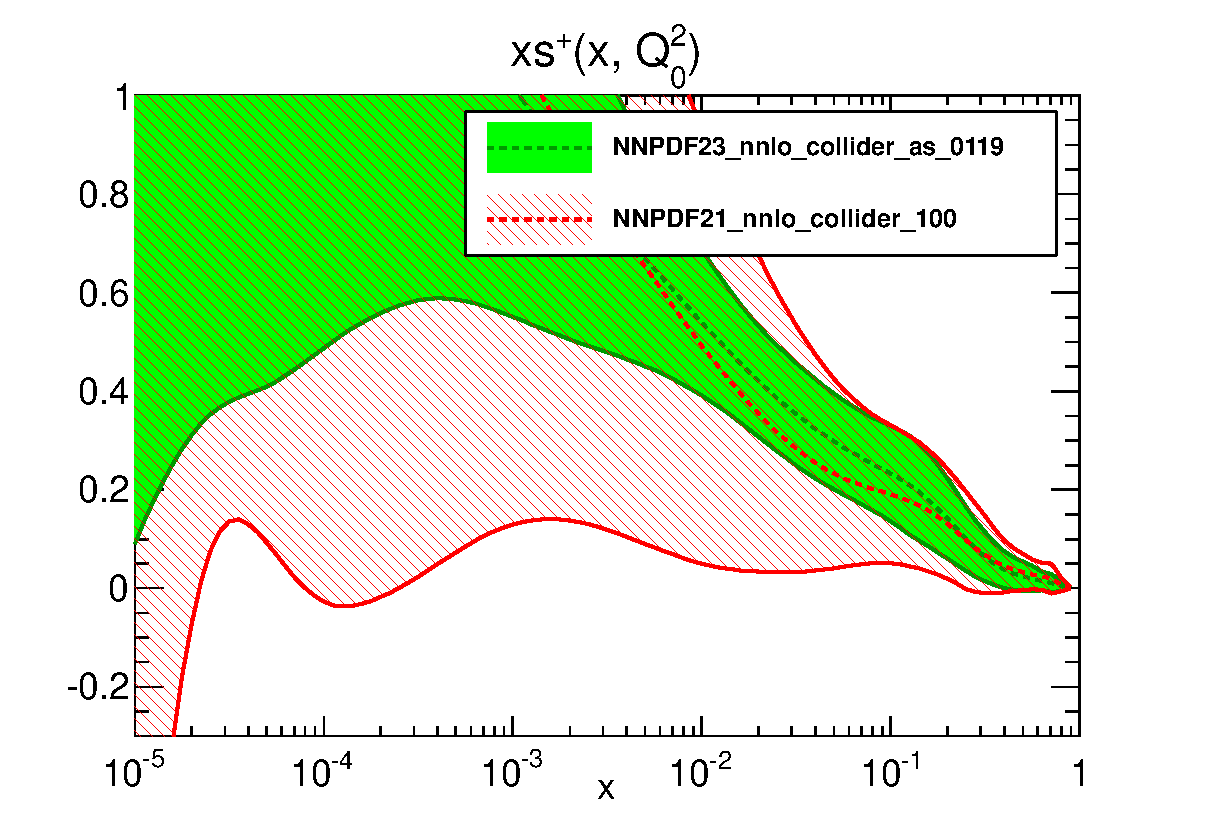
\includegraphics[width=0.5\textwidth]{pdf_xsplus_log_band_comparison_coll.eps}

   \begin{itemize}
   \item<1-> LHC Electroweak measurements in NNPDF2.3 offers substantial constraint. Particularly in the collider only determination which
   previously suffered from a lack of data targeting strangeness.
   \vskip10pt
   \item<1-> Data in 2.3 Collider only determination prefers larger values for total strangeness, although uncertainties remain large.
	\end{itemize}
\end{frame}

\begin{frame}
\frametitle{The strange content of the proton.}

    \begin{columns}
  \begin{column}{0.5\textwidth}
  \begin{center}
     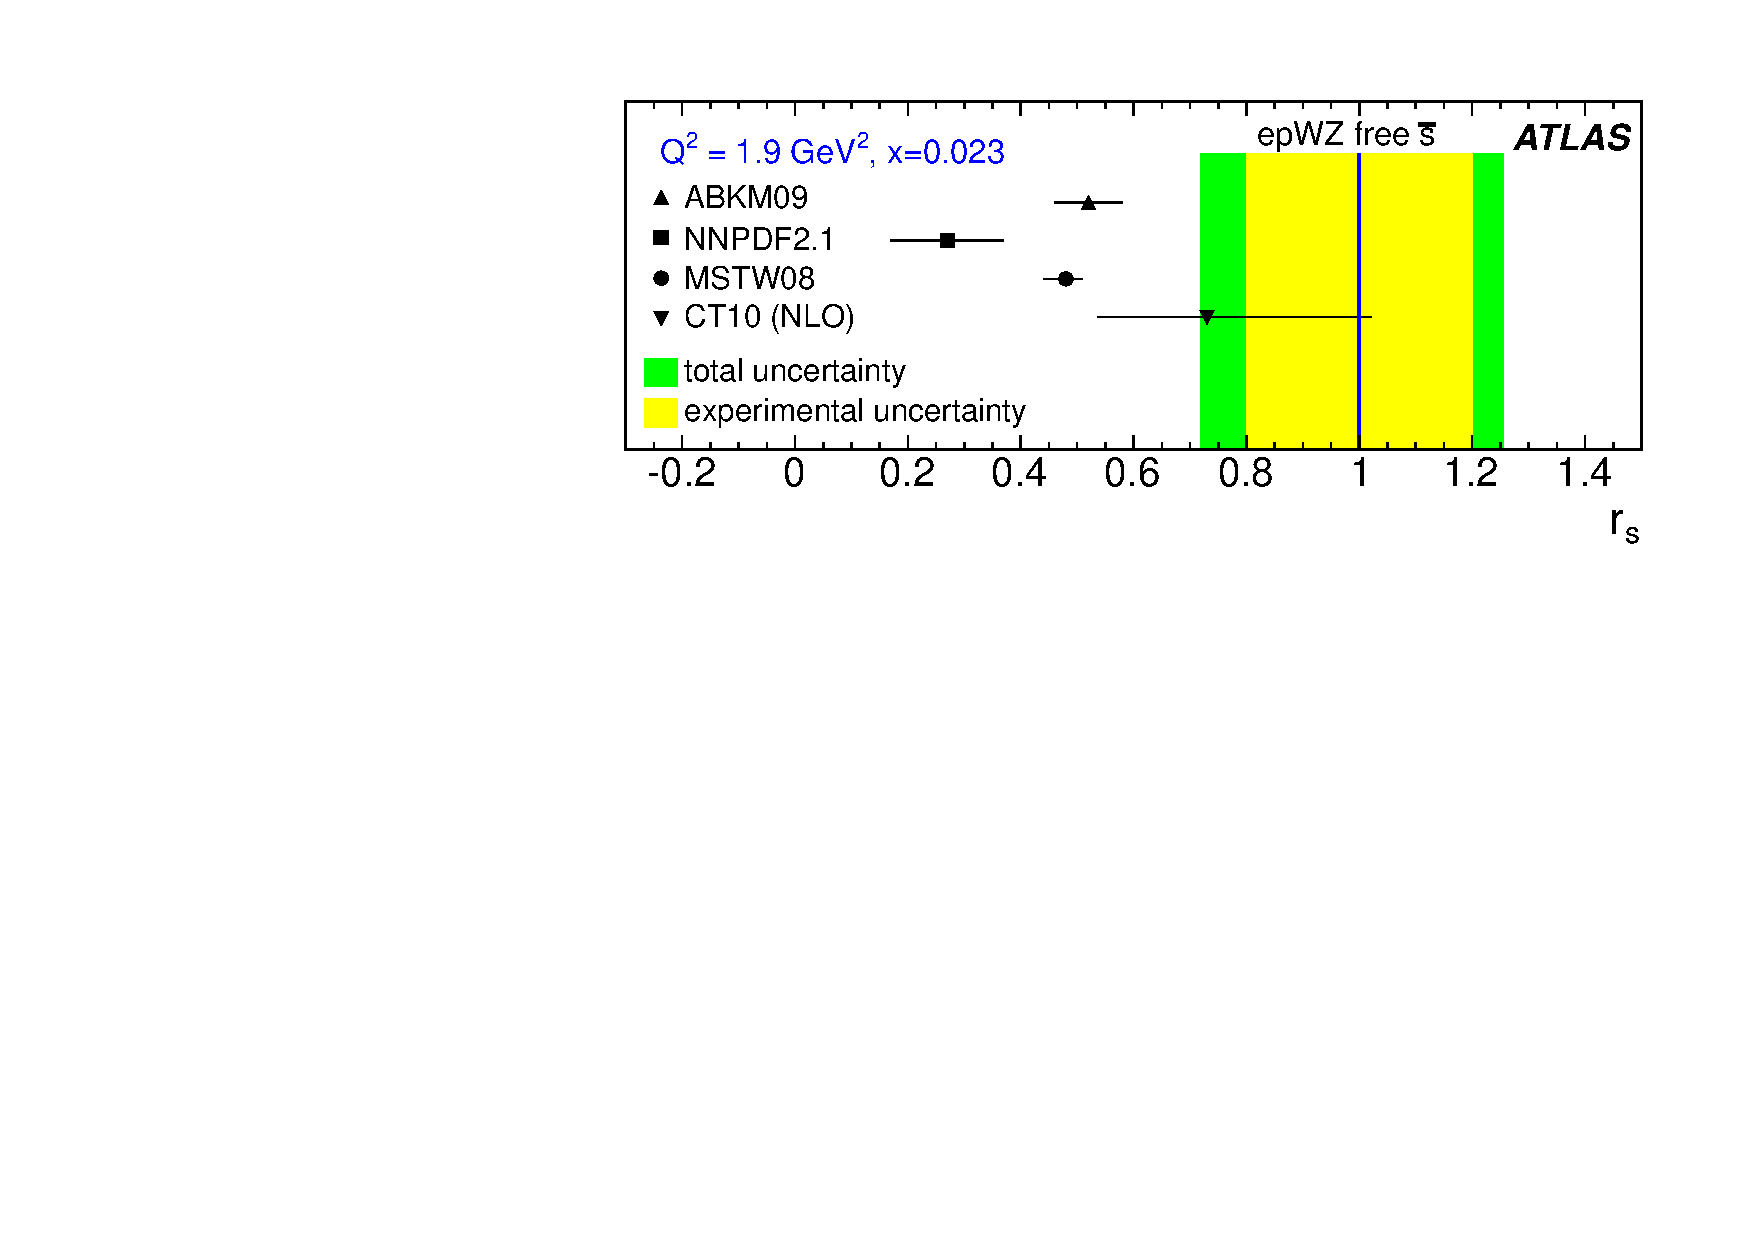
\includegraphics[width=0.8\textwidth]{fig2.pdf}\\
       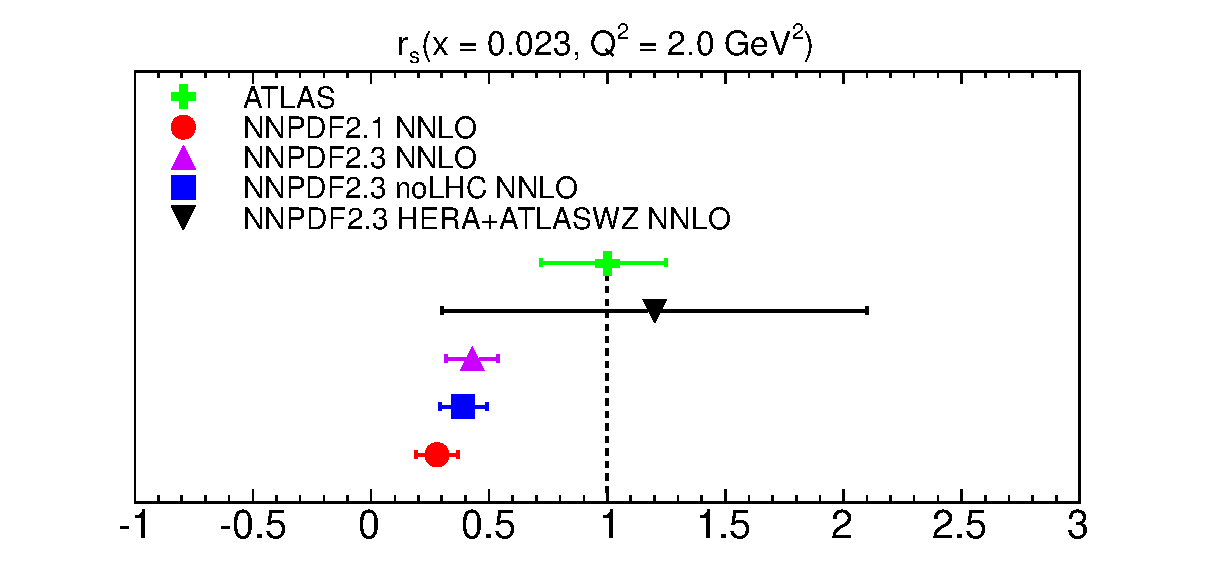
\includegraphics[width=0.8\textwidth]{rs-2.eps}
       \end{center}
               \end{column}
  \begin{column}{0.5\textwidth}

    \begin{center}

   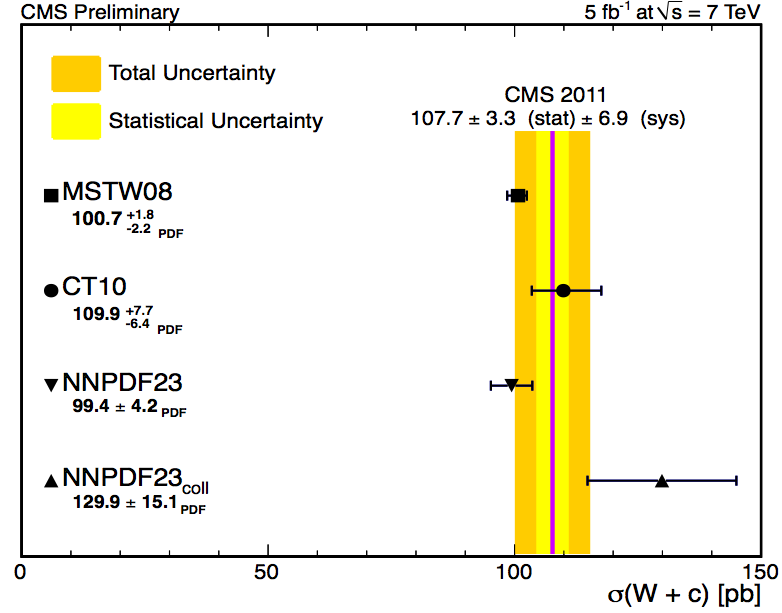
\includegraphics[width=0.9\textwidth]{CMSWc.png}
       \end{center}

   \end{column}
  \end{columns}
            \vskip10pt
  {\small
  \begin{itemize}
\item<1->NNPDF fit to HERA and ATLAS-WZ data finds central
value consistent with ATLAS\footnote{arXiv:1203.4051} determination of $r_s(x) = (s(x) + \bar{s}(x)) / 2d(x)$ within a large uncertainty.
\item<1->Recent CMS\footnote{CMS-SMP-12-002} measurement of $W+c$ consistent with strangeness in global fits.
Slightly disfavours the larger strange sea in NNPDF2.3 Collider only, but consistent within uncertainties.
\end{itemize}

}


\end{frame}


\begin{frame}
\frametitle{PDF Benchmarking}
\textbf{[arXiv:1211.5142] -
Benchmark study of different PDF determinations.}\\
\small{Detailed comparison at common $\alpha_S$ of the most up to date NNLO fits from the ABM, CT, HERAPDF, MSTW and NNPDF collaborations.}

\vskip10pt
     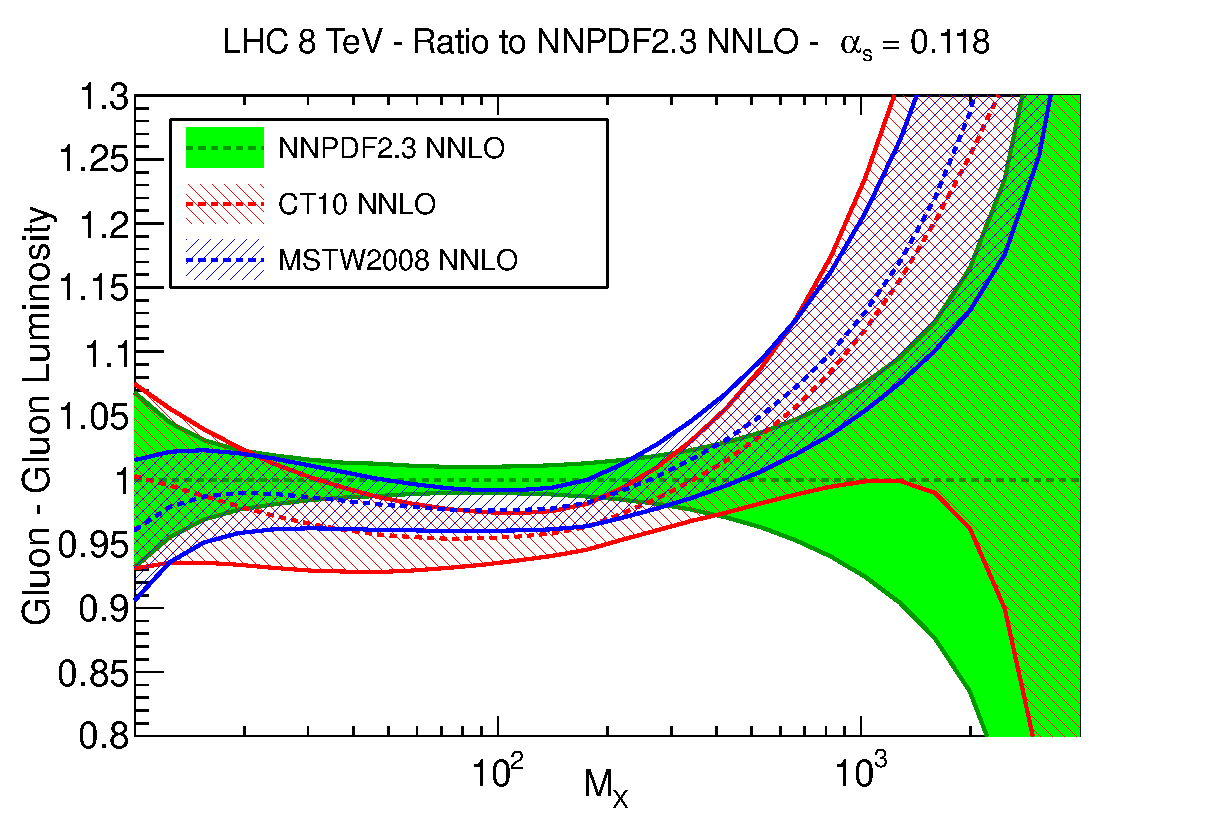
\includegraphics[width=0.5\textwidth]{gg_8tev_as_0118.eps}
 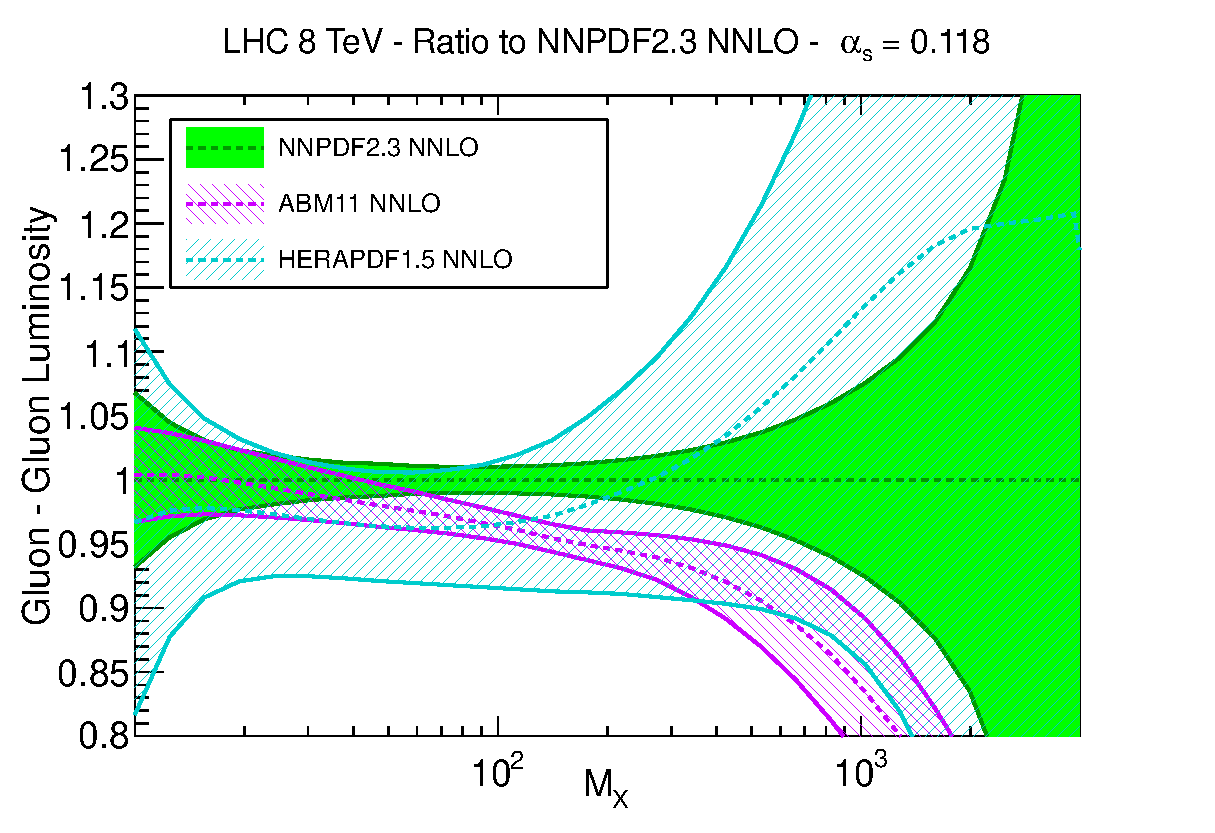
\includegraphics[width=0.5\textwidth]{gg_8tev_as_0118_b.eps}
\vskip10pt
\small{
Reasonable agreement was found between CT, MSTW, NNPDF. \\ \vskip5pt ABM softer large-x gluon and harder quarks.}
\\ \vskip5pt Central values of HERAPDF1.5 NNLO agree with
global fits,  larger uncertainties due to reduced dataset.

\end{frame}

\begin{frame}
     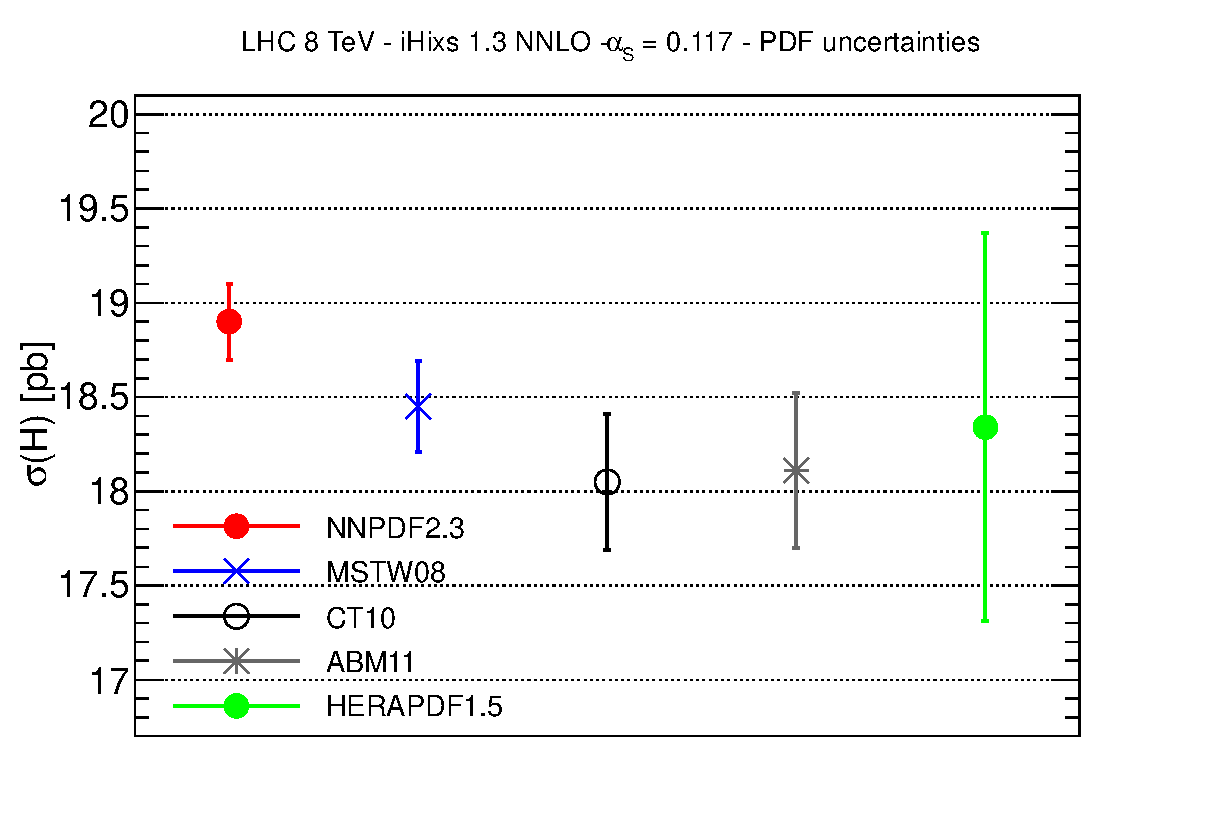
\includegraphics[width=0.5\textwidth]{h8-as0117.eps}
 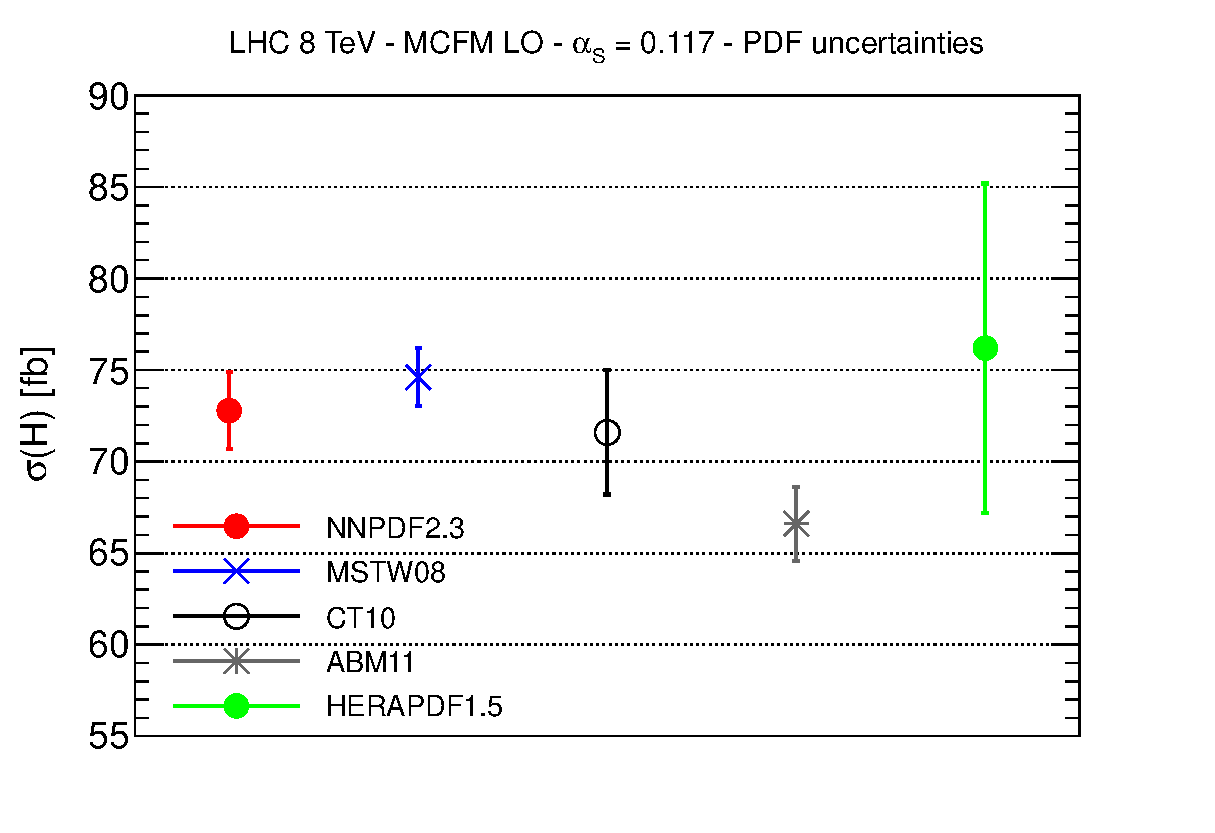
\includegraphics[width=0.5\textwidth]{h8tt-as0117.eps}\\
     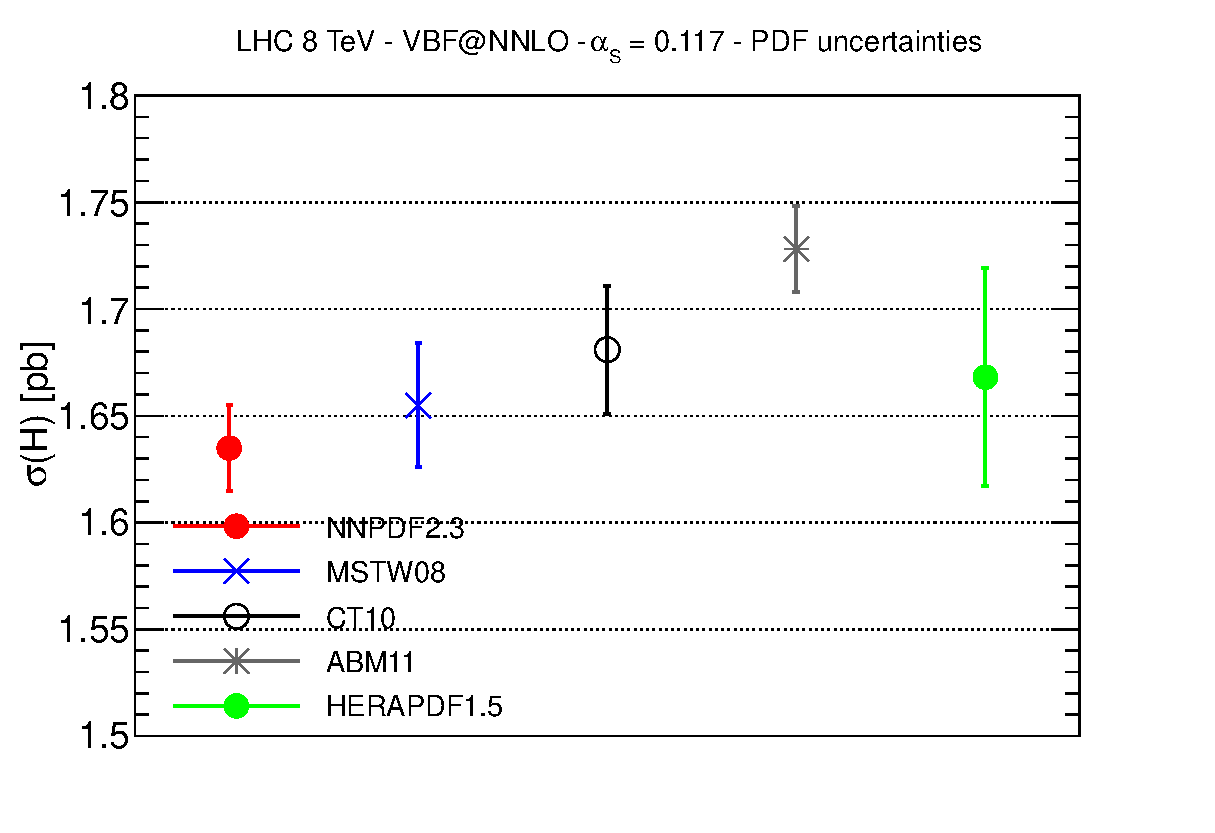
\includegraphics[width=0.5\textwidth]{h8vbf-as0117.eps}
 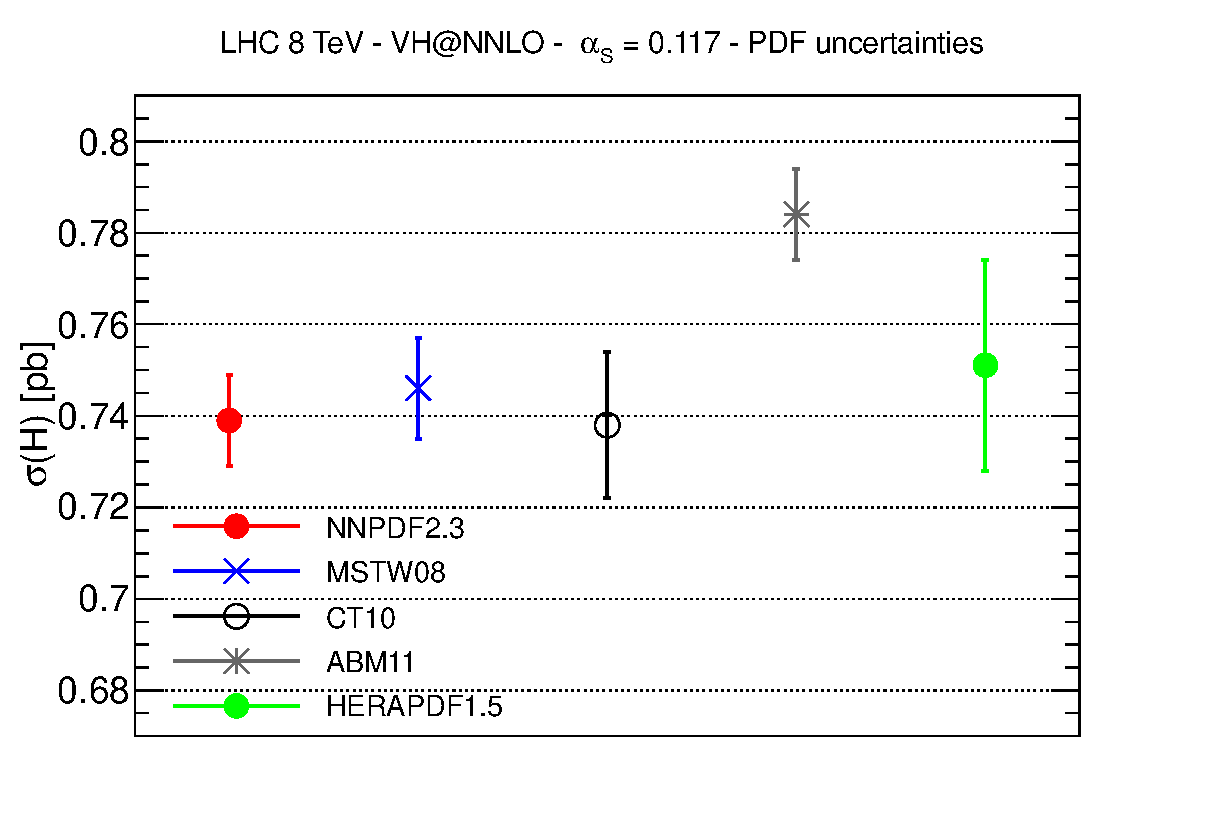
\includegraphics[width=0.5\textwidth]{h8wh-as0117.eps}


\end{frame}

\begin{frame}
\frametitle{Theoretical uncertainties in PDF determination.}
\textbf{[arXiv:1303.1189]} - NNPDF study of contributions to theoretical uncertainty.\\

\begin{itemize}
\item<1-> \textbf{Dynamical Higher Twist}\\
\small NNPDF Fit with higher twist corrections (from ABM determination) indicates modest impact upon PDFs

\item<1-> \textbf{Deuterium nuclear corrections}\\
\small	Potentially affects down quark, fitted from deuterium data. Impact is limited to the $d/u$ ratio in the range $0.1 \le x \le 0.5 $


\end{itemize}

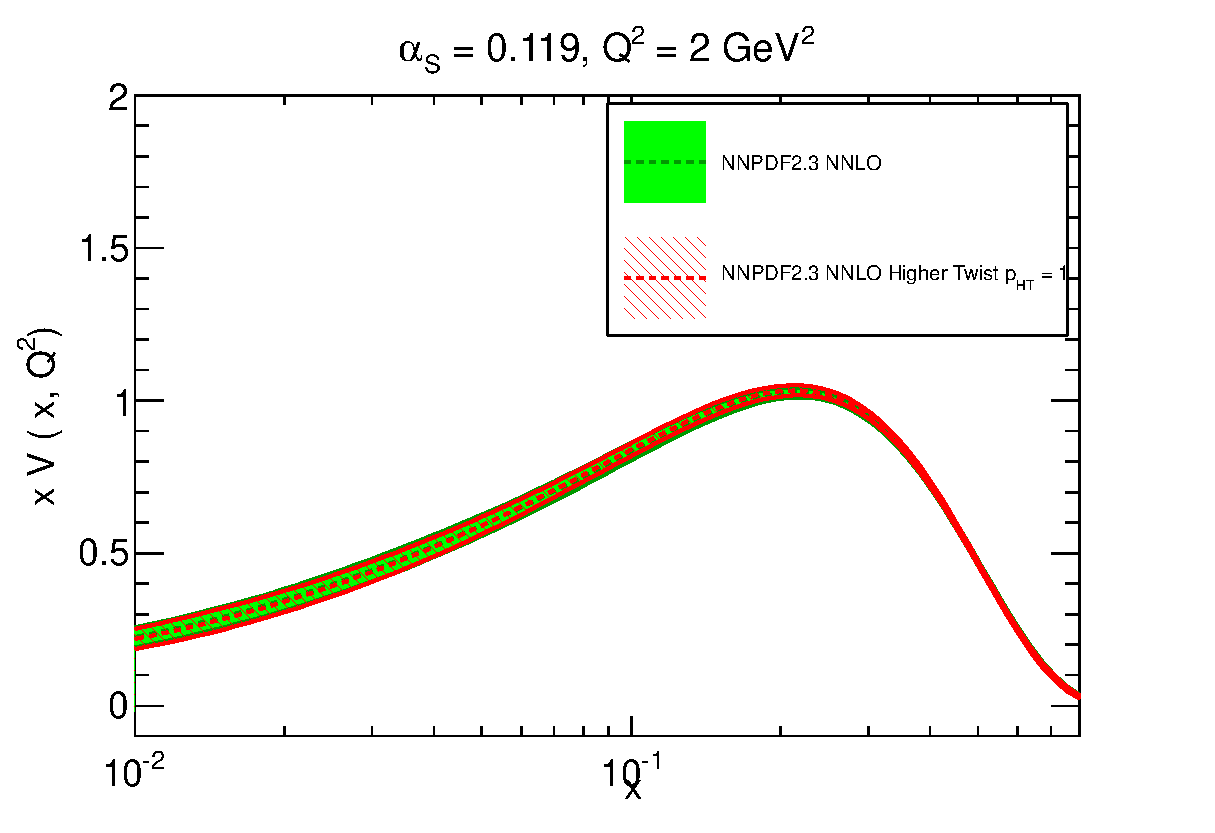
\includegraphics[width=0.5\textwidth]{xvalence-abs-nnpdf-nnpdf23-ref-vs-htp1-q2-2gev2.eps}
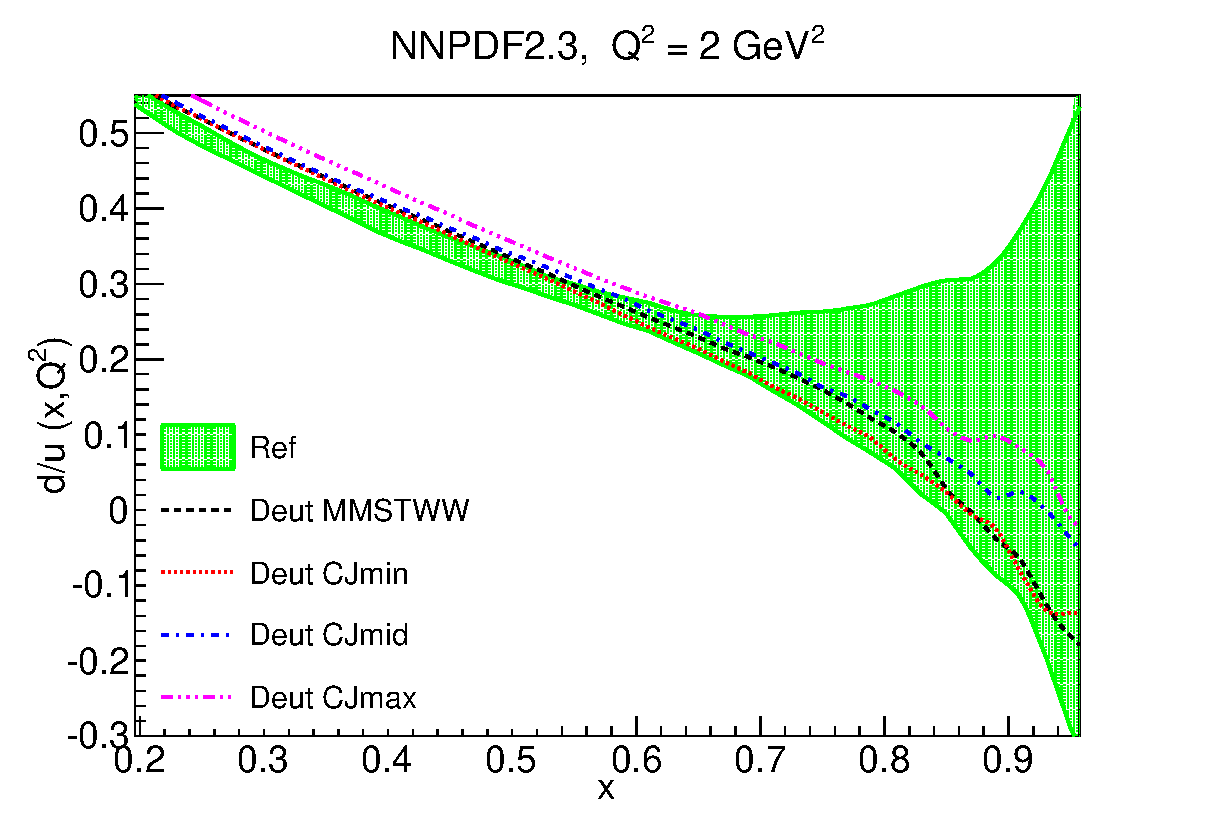
\includegraphics[width=0.5\textwidth]{d_over_u_deut.eps}

\end{frame}

\begin{frame}
\frametitle{Impact of Flavour Number Scheme choice.}

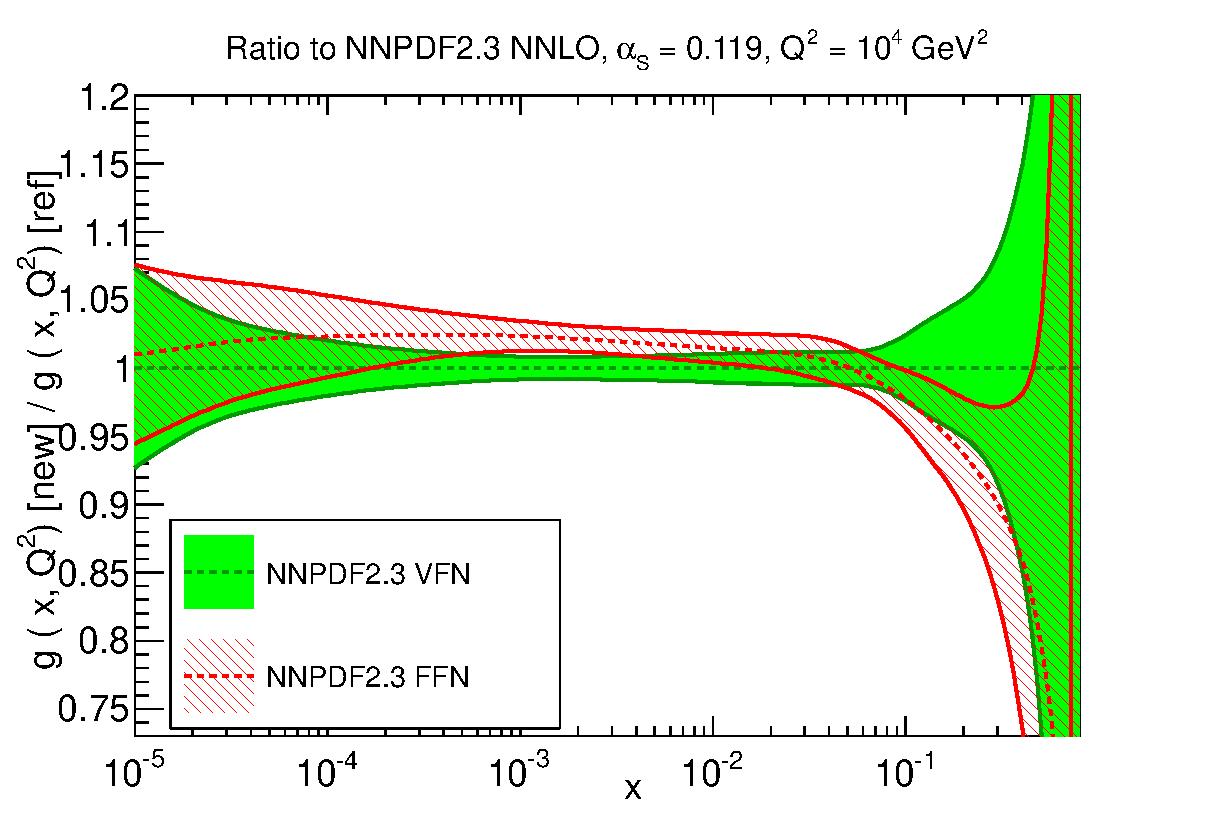
\includegraphics[width=0.5\textwidth]{xg-nnpdf-nnpdf23global-vfn-vs-ffn-10000gev2.eps}
\includegraphics[width=0.5\textwidth]{xsinglet-nnpdf-nnpdf23global-vfn-vs-ffn-10000gev2.eps}

\vskip10pt

\begin{itemize}
\item<1-> \textbf{GM-VFNS vs FFNS}\\
\small		NNPDF fit with a fixed flavour number scheme treatment for DIS observables. Substantial impact observed in PDF central values.
\vskip5pt
The FFN quarks increase at medium to low-x\\
The FFN gluon becomes softer at high-$x$.
\vskip5pt
\end{itemize}

\end{frame}

\begin{frame}
\frametitle{Impact of FFN Scheme}
\begin{center}
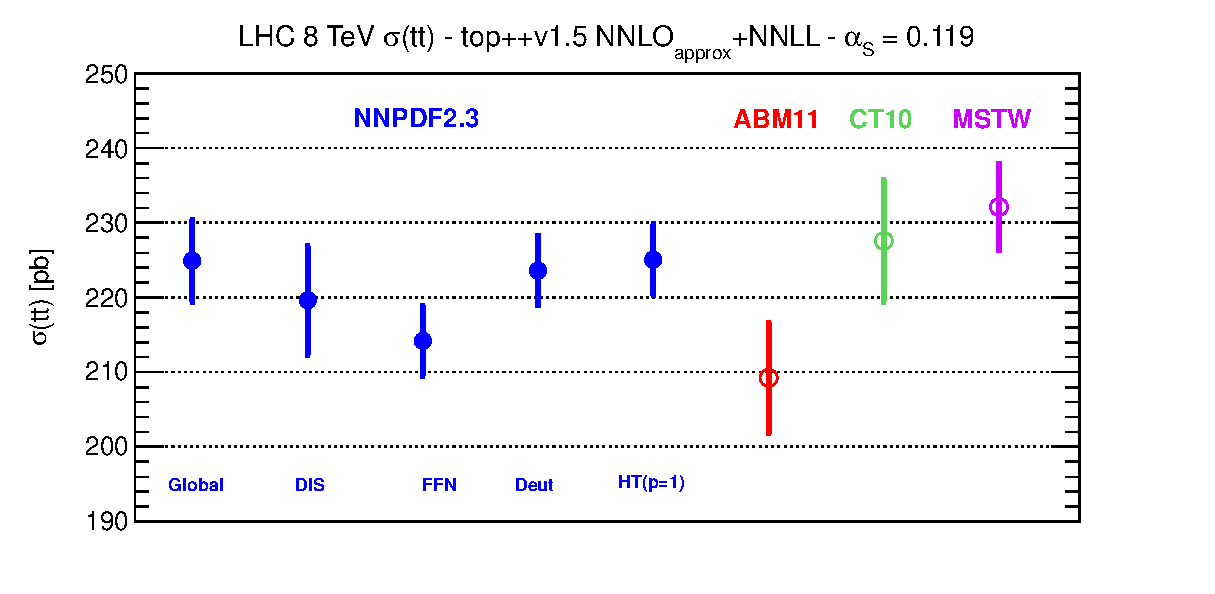
\includegraphics[width=0.7\textwidth]{tt8.eps}\\
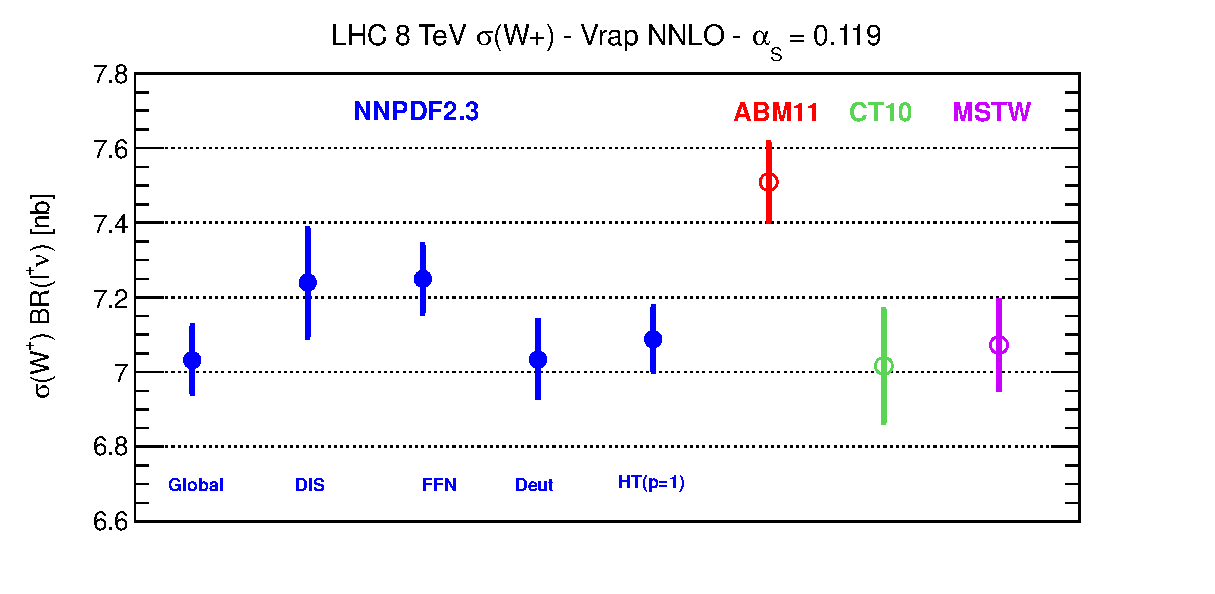
\includegraphics[width=0.7\textwidth]{wp8.eps}
\end{center}
\end{frame}

\begin{frame}

\frametitle{Towards NNPDF3.0}

\underline{Challenges}
\begin{itemize}
\item<1-> \textbf{Predictions for LHC data are computationally rather expensive.}\\
		- A fast fitting framework is required.
\item<1-> \textbf{New datasets from the LHC and HERA are becoming available.} \\
		- The ability to rapidly implement and assess the impact of new data is vital.
\item<1-> \textbf {Fitting methodology should be analysed in the light of new data.} \\
		- Is our current methodology doing the best job it can?

\end{itemize}

\vskip20pt

\small A new NNPDF code is under development, built from scratch to support rapid iteration.
\begin{itemize}
\item<1-> Faster fits means more aggressive minimisation, more scope for Methodological surveys.
\item<1-> Code is written in modern C++ to aid flexibility and maintainability.
\item<1-> Rewrite provides an in-depth cross check of the implementation.
\end{itemize}

\end{frame}

\begin{frame}
\frametitle{Towards NNPDF3.0}
\begin{center}
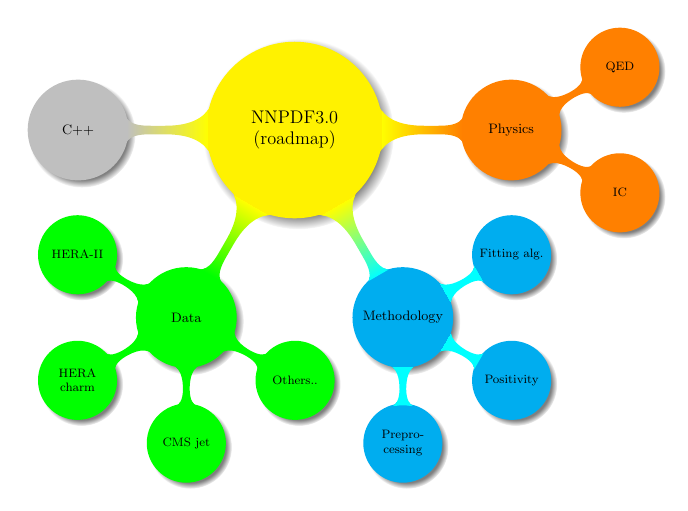
\begin{tikzpicture}   [scale=0.55,transform shape]   \path[mindmap, concept color=yellow,text=black,     every node/.style={concept, circular drop shadow}]
node[concept] {NNPDF3.0 (roadmap)}   [clockwise from=0]
child[concept color=orange]{ node[concept] {Physics} [clockwise from=30]
child[concept color=orange] { node[concept] {QED}       [clockwise from=0]
}
child[concept color=orange] { node[concept] {IC}       [clockwise from=0]
}
}
child[concept color=cyan]{
node[concept] {Methodology}      [clockwise from=30]
child[concept color=cyan] { node[concept] {Fitting alg.}       [clockwise from=0]
}
child[concept color=cyan] { node[concept] {Positivity}       [clockwise from=0]
}
child[concept color=cyan] { node[concept] {Prepro- cessing}       [clockwise from=0]
}
}
child[concept color=green]{ node[concept] {Data} [clockwise from=-30]
child[concept color=green] { node[concept] {Others..}       [clockwise from=0]
}
child[concept color=green] { node[concept] {CMS jet}       [clockwise from=0]
}
child[concept color=green] { node[concept] {HERA charm}       [clockwise from=0]
}
child[concept color=green] { node[concept] {HERA-II}       [clockwise from=0]
}
}
child[concept color=lightgray]{ node[concept] {C++}
};
\end{tikzpicture}
\par\end{center}
\end{frame}

%
%	\vskip20pt
%\underline{Preliminary fits with new data}
%\begin{itemize}
%
%\item<1-> \textbf{Updated measurements from HERA.}\\
%	- Inclusive DIS, $F^2_c$ datasets available from HERA collaborations.
%\end{itemize}
%
\begin{frame}
\frametitle{New data - HERA-II DIS}

\begin{columns}
  \begin{column}{0.5\textwidth}
     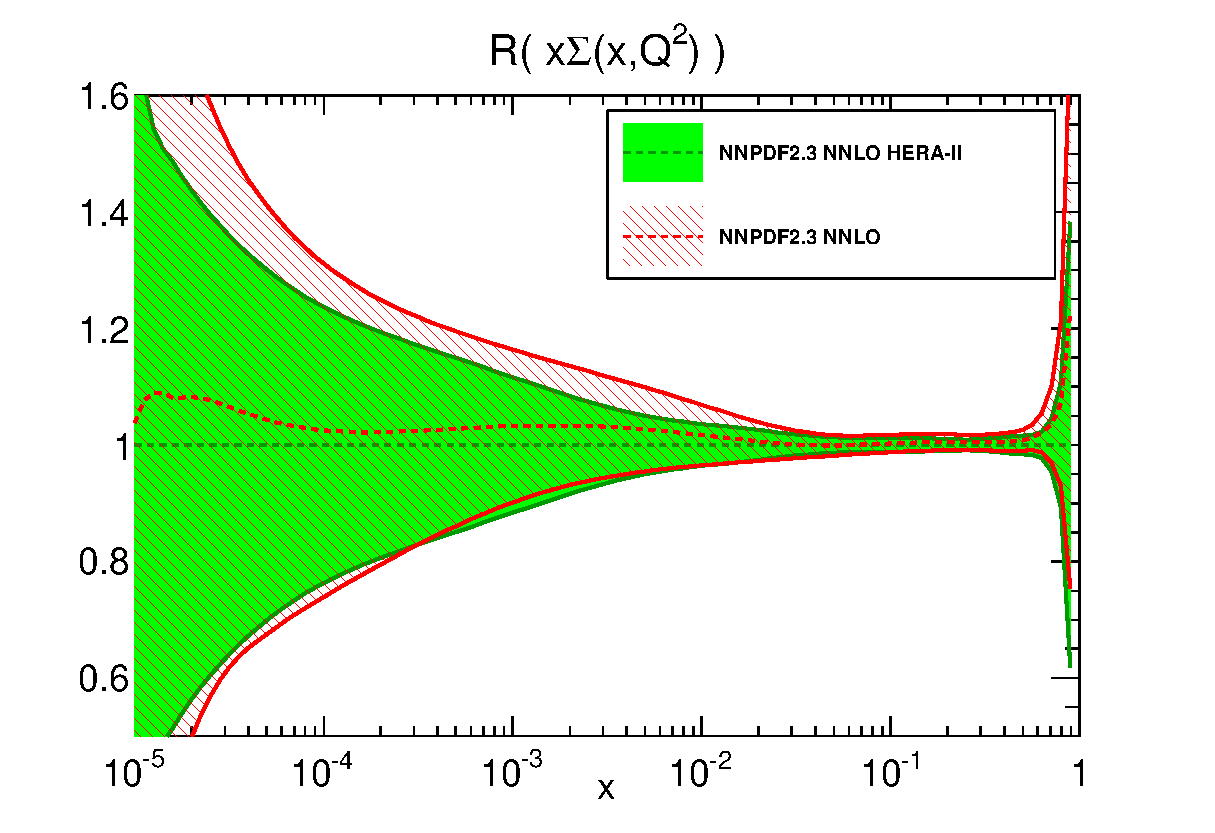
\includegraphics[width=1.0\textwidth]{pdf_xSigma_log_ratio_HERAII.eps}\\

\end{column}
  \begin{column}{0.5\textwidth}

  \small  {\textbf{Preliminary Fits to HERA-II Inclusive DIS Datasets.} }
\vskip5pt
Large new DIS datasets from the ZEUS and H1 collaborations.
\vskip5pt
Over \textbf{600} new data points demonstrate excellent consistency in global
fit, providing constraint particularly for the singlet PDF.
\vskip5pt
PDF distances demonstrate this consistency. A distance of $d = 10$ implies
a shift by $1$-$\sigma$.

\end{column}
\end{columns}

     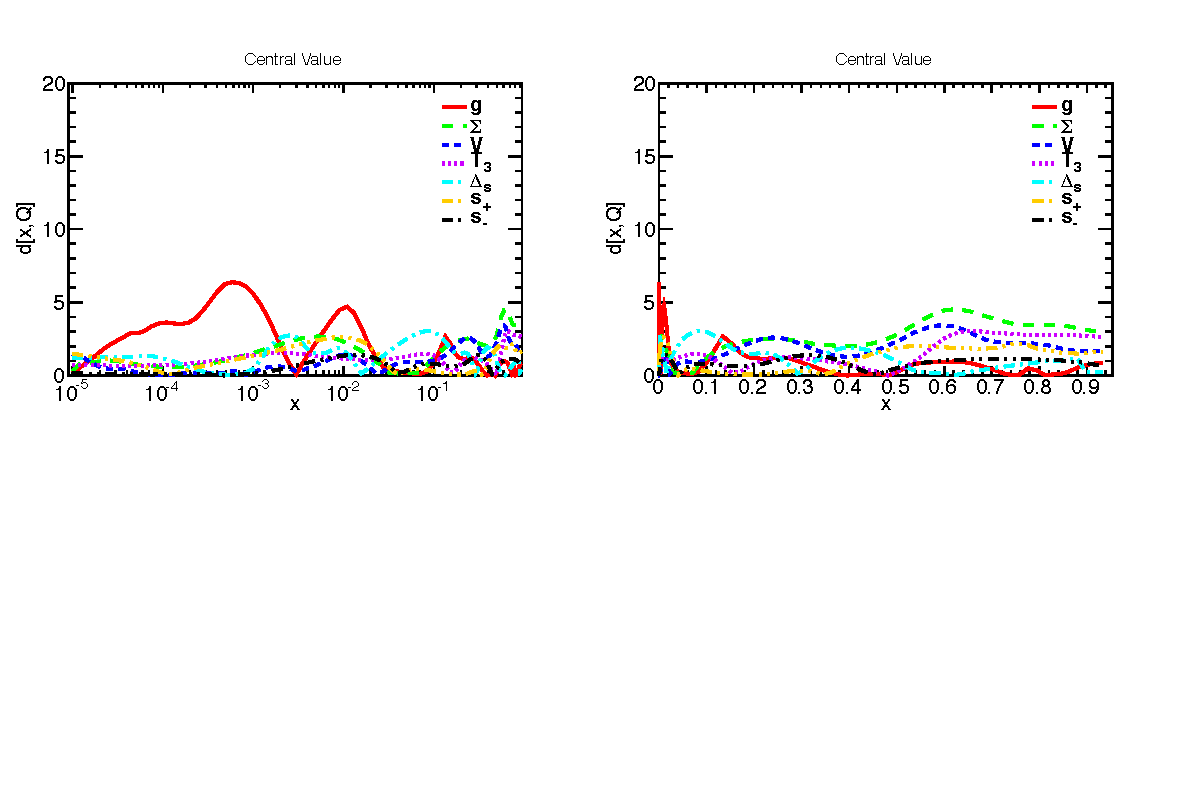
\includegraphics[width=1.0\textwidth]{HERA-II_distancesv2.pdf}

\end{frame}


\begin{frame}
\frametitle{New data - HERA Combined $F^2_c$}
\textbf{[arXiv:1211.1182] - ZEUS and H1 Combination $F^2_c$ data.}\\ \vskip5pt
Supersedes separate datasets used in previous NNPDF fits, providing additional information on data correlations.
\vskip10pt
    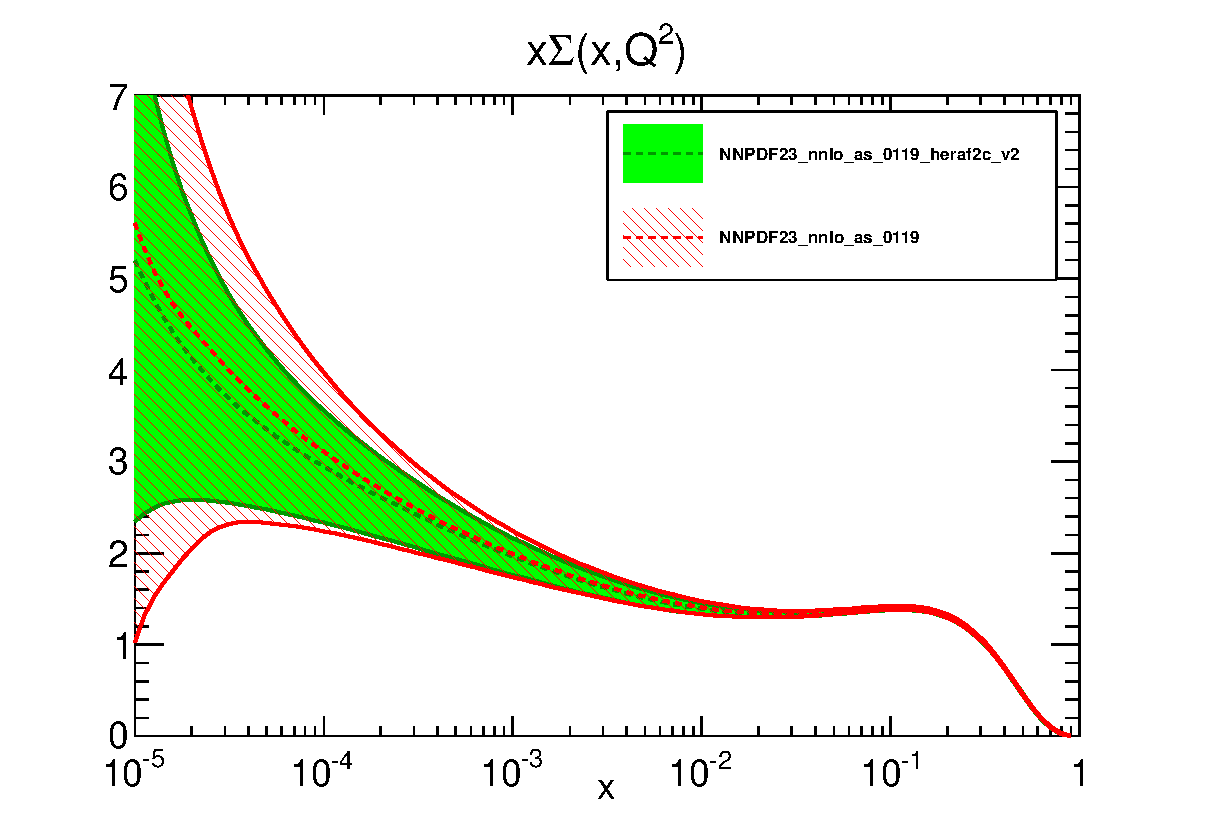
\includegraphics[width=0.5\textwidth]{pdf_xSigma_log_f2c.eps}
        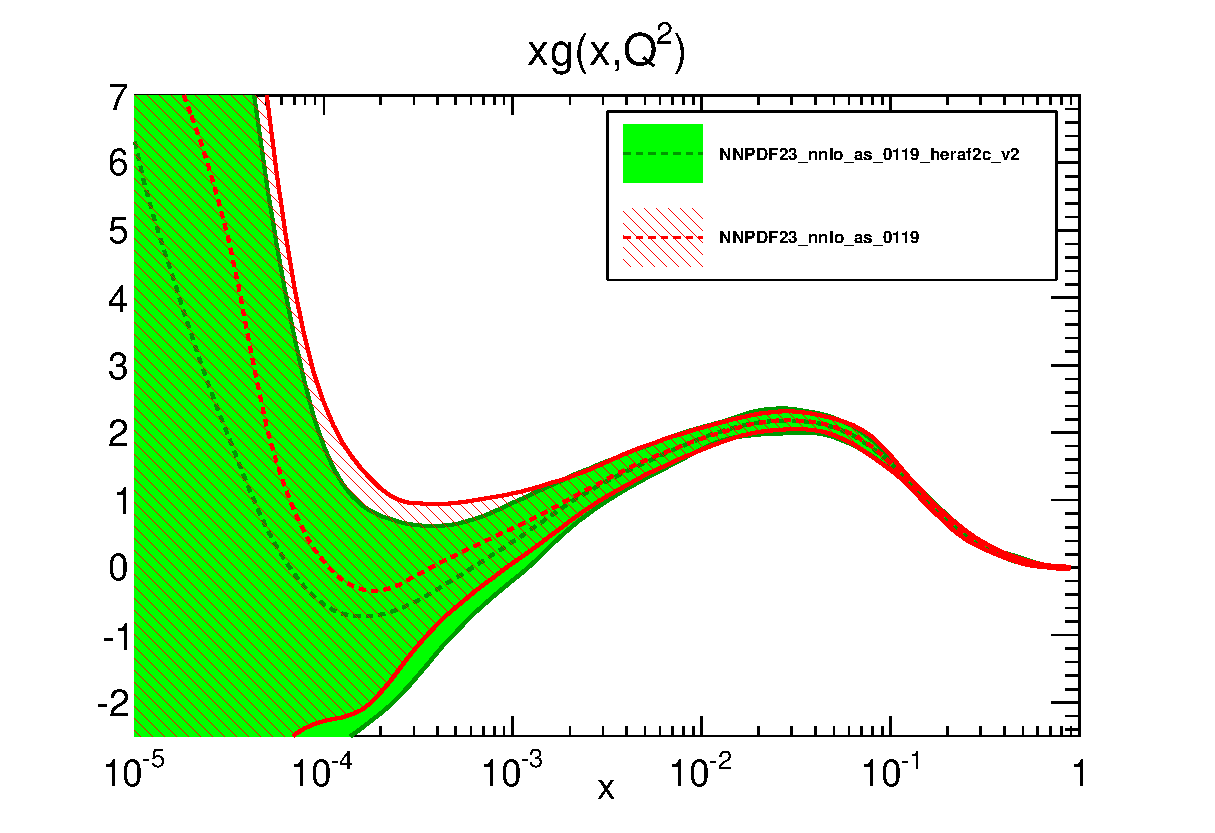
\includegraphics[width=0.5\textwidth]{pdf_xg_log_f2c.eps}
        \vskip10pt
Introducing the extra correlations has a generally modest impact, restricted to the singlet and gluon distributions.
\end{frame}




\begin{frame}
\frametitle{Methodology: Closure tests}
How do we ensure that our fit minimises \emph{bias}?\\
\emph{Related studies by Thorne-Watt [arXiv:1205.4024]}
\vskip15pt
\underline{Perform a \textbf{Closure Test}}:

\begin{itemize}
\item<1-> \textbf{Generate artificial pseudo-data based upon a known PDF distribution.}\\
		\small Pseudodata generated according to NLO pQCD. Dataset is therefore free of internal inconsistencies.
		\vskip15pt

\item<1-> \textbf{Simulate experimental noise in the pseudodata. }\\
			\small Data points perturbed according to multi-gaussian distribution defined by the experimental
			covariance matrix.
			\vskip15pt
\item<1-> \textbf{Perform a full PDF fit to the pseudo-dataset.}\\
		\small Closure fit should recover generating PDF up to the level of experimental uncertainty.
\end{itemize}

\end{frame}

\begin{frame}
\frametitle{Methodology: Closure tests}


\small  {\textbf{Preliminary NNPDF closure test fits.} }\\
First closure tests performed with NNPDF C++ code to a NLO fit with a global dataset.
\vskip5pt
     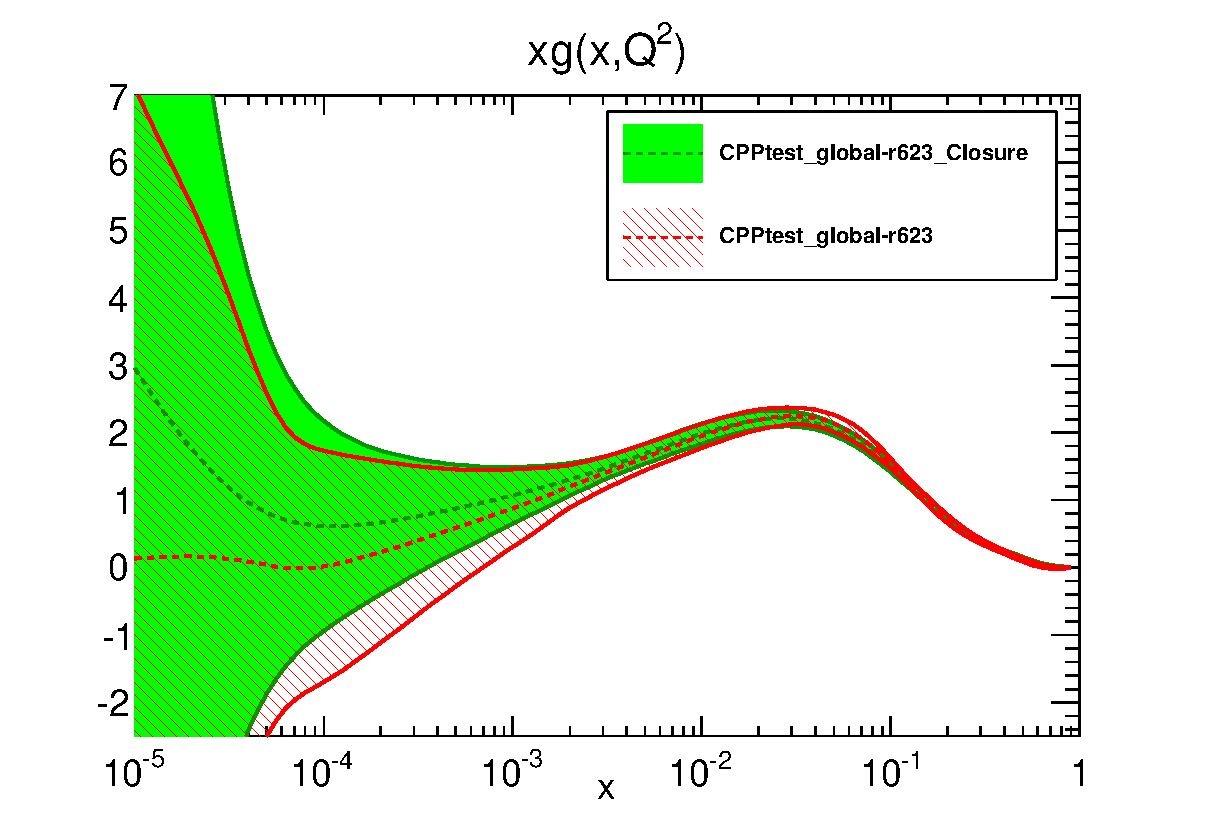
\includegraphics[width=0.5\textwidth]{pdf_xg_log.eps}
     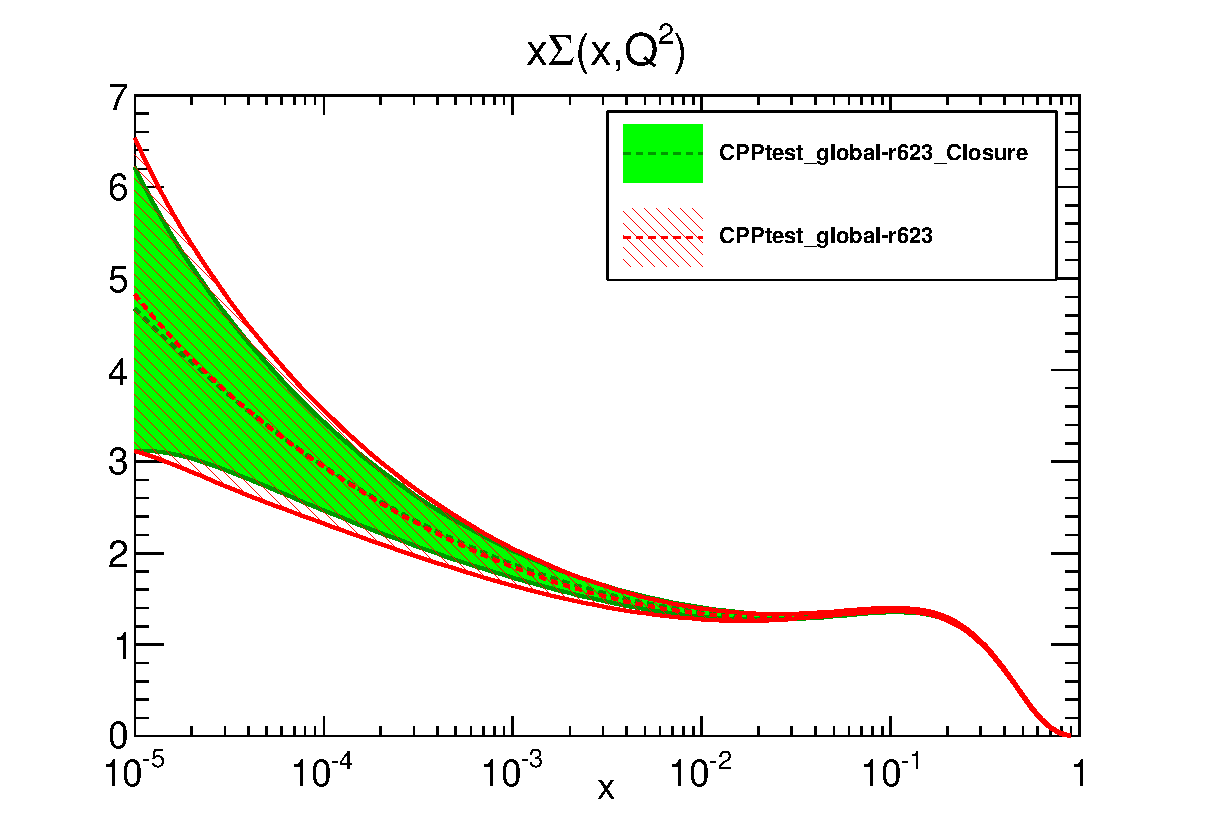
\includegraphics[width=0.5\textwidth]{pdf_xSigma_log.eps}

     \vskip5pt
\small{ Early closure test fits demonstrate good reproduction of the generating function, accurate up to experimental error. }
\vskip10pt
\small{Reproduction of uncertainty is particularly interesting. Lack of data inconsistency does not appear to lead to significant change in the resulting uncertainties. }
\vskip10pt
\small{The NNPDF methodology can be consistently applied to experimental data and theoretically perfect pseudodata without the need for tolerance.}

\end{frame}

\begin{frame}
\frametitle{Preliminary closure tests - fit quality}

 \begin{columns}
  \begin{column}{0.5\textwidth}
  \begin{center}  \textbf{Pseudodata} \end{center}
     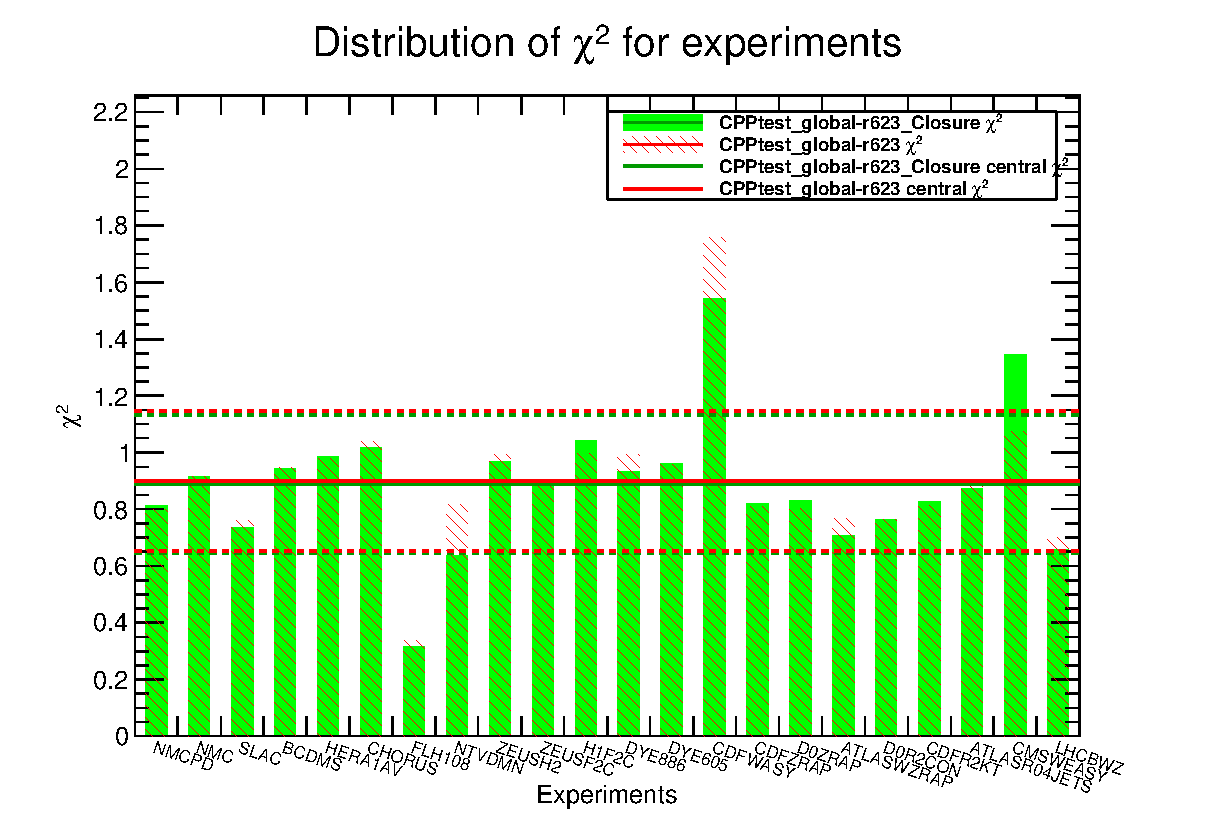
\includegraphics[width=1.0\textwidth]{chi2_histo_nnpdf1.eps}
     \end{column}
       \begin{column}{0.5\textwidth}
         \begin{center}  \textbf{Experimental data} \end{center}

     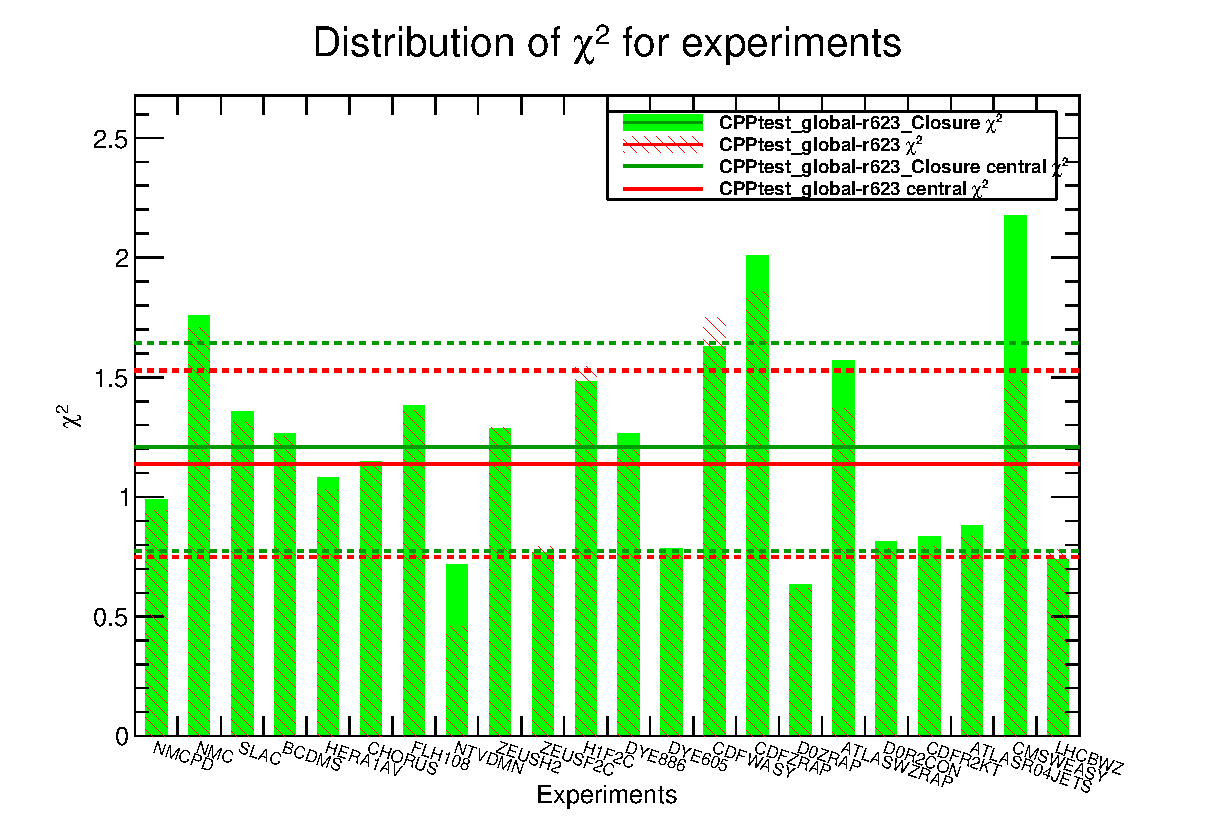
\includegraphics[width=1.0\textwidth]{chi2_histo_nnpdf2.eps}
     \end{column}
     \end{columns}
     \vskip10pt
     \begin{itemize}
     \item<1-> The $\chi^2$ value for each dataset is assessed both for the artificial pseudodata, and for the real experimental data.
     \item<1-> Closure test fit demonstrates self consistency of the NNPDF procedure.
     \end{itemize}


\end{frame}
%
%\begin{frame}
%
%
%\frametitle{Preliminary closure tests - MSTW08 Closure }
%
%{\small
%Can we run a closure test to an input PDF determined by a \textbf{different methodology}? }
%\begin{itemize}
%\item<1> \small Preliminary NNPDF C++ fit to pseudodata generated by \textbf{MSTW08} NLO.
%\end{itemize}
%
% \begin{columns}
%  \begin{column}{0.5\textwidth}
%  \begin{center}  \textbf{Pseudodata} \end{center}
%     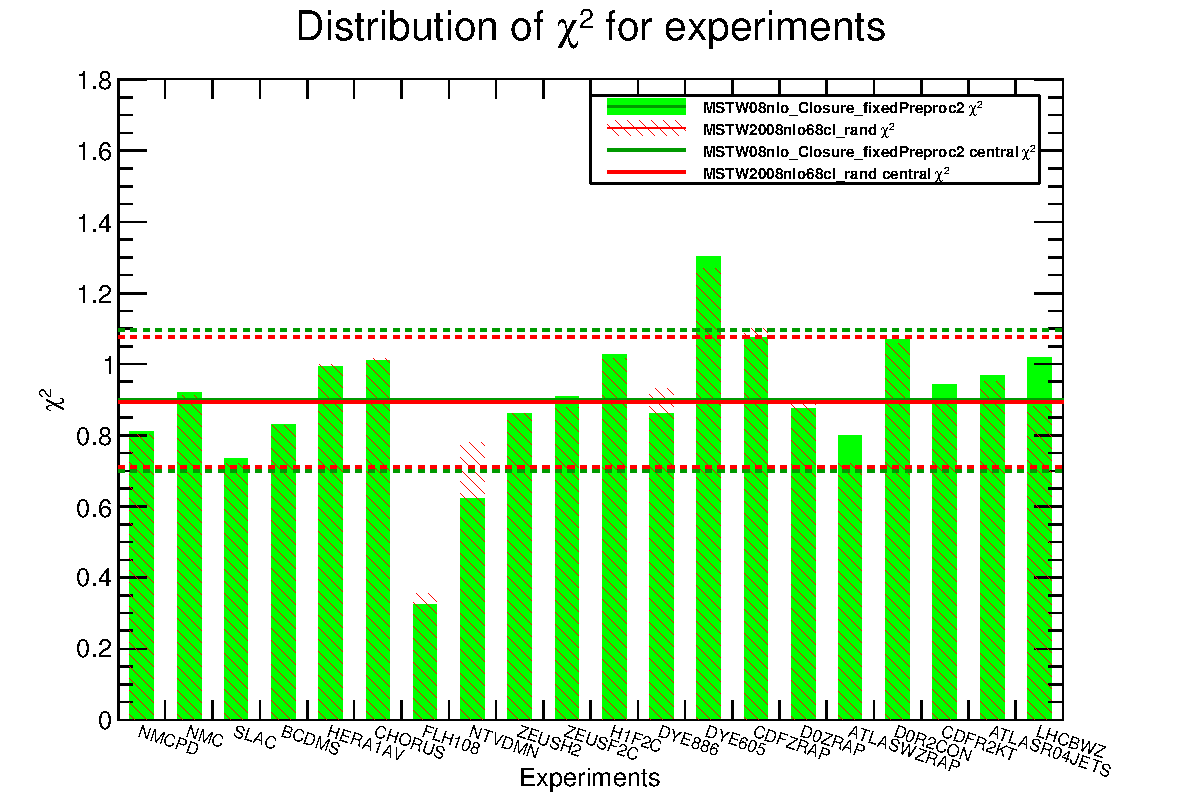
\includegraphics[width=1.0\textwidth]{chi2_histo_mstw1.eps}
%     \end{column}
%       \begin{column}{0.5\textwidth}
%         \begin{center}  \textbf{Experimental data} \end{center}
%
%     \includegraphics[width=1.0\textwidth]{chi2_histo_mstw2.eps}
%     \end{column}
%     \end{columns}
%
%\begin{itemize}
%\item<1-> The closure test fit is able to reproduce the $\chi^2$ values of MSTW08 to both the pseudo and experimental datasets to a good accuracy.
%\item<1-> Further closure testing will help guide the development of the NNPDF C++ code.
%\end{itemize}
%
%
%\end{frame}

\begin{frame}
\frametitle{Summary and Outlook}




\underline{Current Status}

\begin{itemize}
	\item<1-> \textbf{NNPDF2.3}\\
	{ \small The NNPDF2.3 family of fits provide a determination of parton distribution functions with a global dataset, including a sizeable LHC contribution. }
	\vskip10pt
	{\small Measurements from the LHC and HERA will provide interesting further constraints upon PDFs, particularly in collider only determinations.}
\end{itemize}
\vskip10pt

\underline{Looking Forward}\\
A great deal of progress in NNPDF determinations across many fronts.
\begin{itemize}
	\item<1-> \textbf{Progress towards the next global NNPDF set}\\

	\begin{itemize}
	\item<1-> New fitting framework developed from scratch in C++.
	\item<1-> Preliminary methodological studies by Closure Testing.
	\item<1-> Impact of new HERA combinations upon NNPDF2.3 studied.
	\item<1-> Plenty of new data to come (e.g CMS Inclusive Jets, $W+c$).
	\end{itemize}

	\item<1-> \textbf{New Results for PDFs with QED Corrections, and polarised NNPDFs}\\
	{ \small  see talks by S.Carrazza, E.Nocera.}
\end{itemize}


\end{frame}

\begin{frame}
    \begin{center}
      BACKUPS
    \end{center}
\end{frame}


\begin{frame}
\frametitle{Including new experimental data - reweighting}
How can we add new LHC data to an existing parton set?

\begin{itemize}
		\item<1->Reweight existing Monte Carlo parton set.\\
\end{itemize}
Each replica in the set is assigned a weight based upon it's $\chi^2$ to the new data.
\be \langle\mathcal{O}\rangle_{\mathrm {new}}=\smallfrac{1}{N}\,\sum_{k=1}^{N}w_k\mathcal{O}[f_k], \quad\quad w_k \propto
(\chi^{2}_k)^{(n-1)/2}
e^{-\frac{1}{2}\chi^{2}_k}  \ee
\begin{itemize}
		\item<1-> Application: NNPDF2.2 Parton Set   \hfill {\color{blue} [arXiv:1012.0836]}\\
		LHC Electroweak data added by Bayesian Reweighting
\end{itemize}
\vskip10pt

However, reweighting method is impractical for large/constraining data sets.
 Number of effective replicas reduced after reweighting: \be N_{\textrm{ eff}} \equiv \exp \left(\frac{1}{N_{\mathrm{rep}}}\sum_{k=1}^{N_{\mathrm{rep}}}w_k\ln(N_{\mathrm{rep}}/w_k)\right)\ee

\end{frame}


\begin{frame}
\frametitle{Including new experimental data - refitting}
How can we efficiently include LHC data into a full refit?

\underline{Tools}: APPLgrid/FastNLO projects

\begin{itemize}
\item<1-> Precompute and store MC Weights on an interpolation grid
\end{itemize}
\begin{equation}
\label{eq:applconv}
\sigma = \sum_p \sum_{l=0}^{N_{\mathrm{sub}}} \sum_{\alpha,\beta}^{N_x} \sum_{\tau}^{N_{Q}}
W_{\alpha\beta\tau}^{(p)(l)} \, \left( \frac{\alpha_s\left(Q^2_{\tau}\right)}{2\pi}\right)^{p}
F^{(l)}\left(x_{\alpha}, x_{\beta},  Q^2_{\tau}\right)
\end{equation}
PDF Evolution in the FastKernel method is a similar procedure,
\be f_i(x_{\alpha},Q^2_\tau) =  \sum_\beta^{N_{x}} \sum_{j}^{N_{\mathrm{pdf}}} A^{\tau}_{\alpha\beta ij}N^0_j(x_{\beta} )\ee
\underline{Idea}: Combine weight grids with evolution grids

  \be \sigma= \sum_{\alpha,\beta}^{N_x}\sum_{i,j}^{N_{\mathrm{pdf}}} \sigma_{\alpha\beta i j}N_i^0(x_\alpha)N_j^0(x_\beta)\ee
 \begin{itemize}
\item<1-> Precomputing all $Q^2$ dependence leads to extremely efficient calculations.
\end{itemize}\end{frame}

\begin{frame}
\frametitle{NNPDF2.3 Collider only vs NNPDF2.3}
   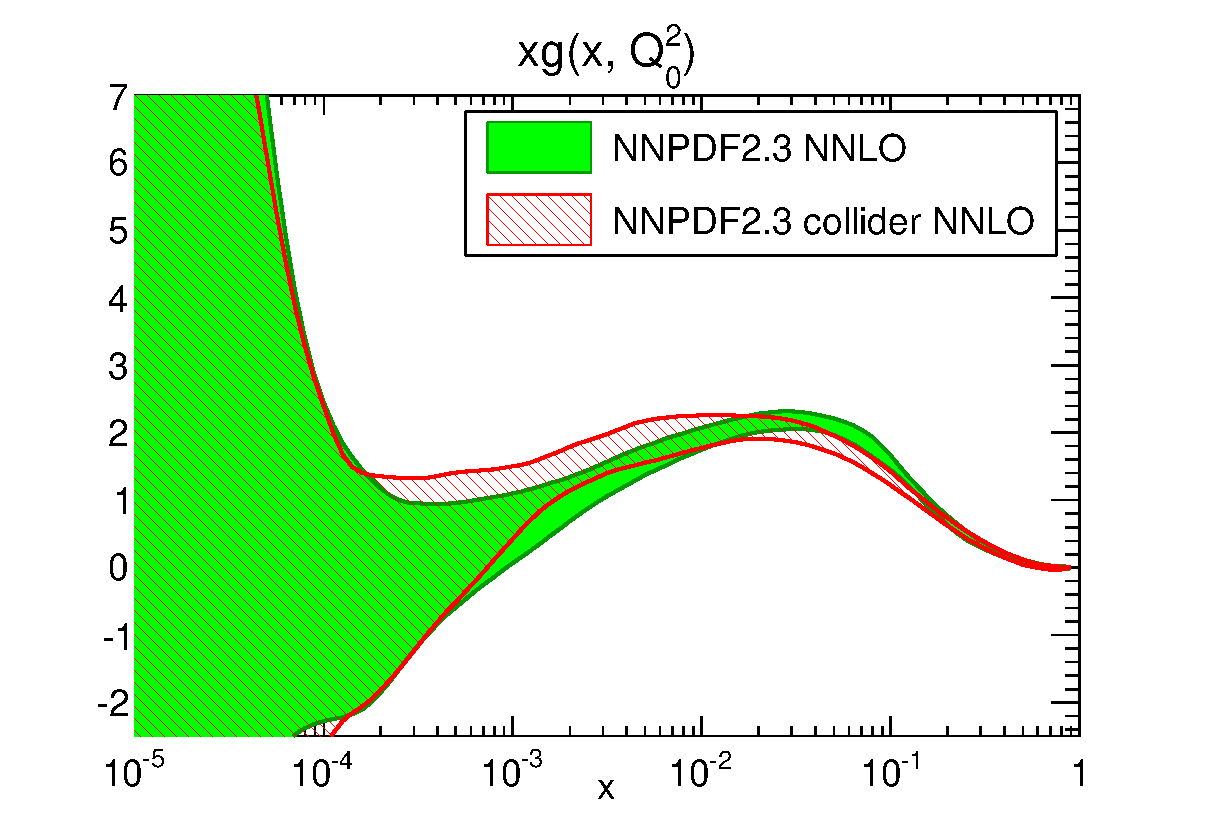
\includegraphics[width=0.5\textwidth]{xg_Q_2_log-23-vs-23coll-nnlo.eps}
 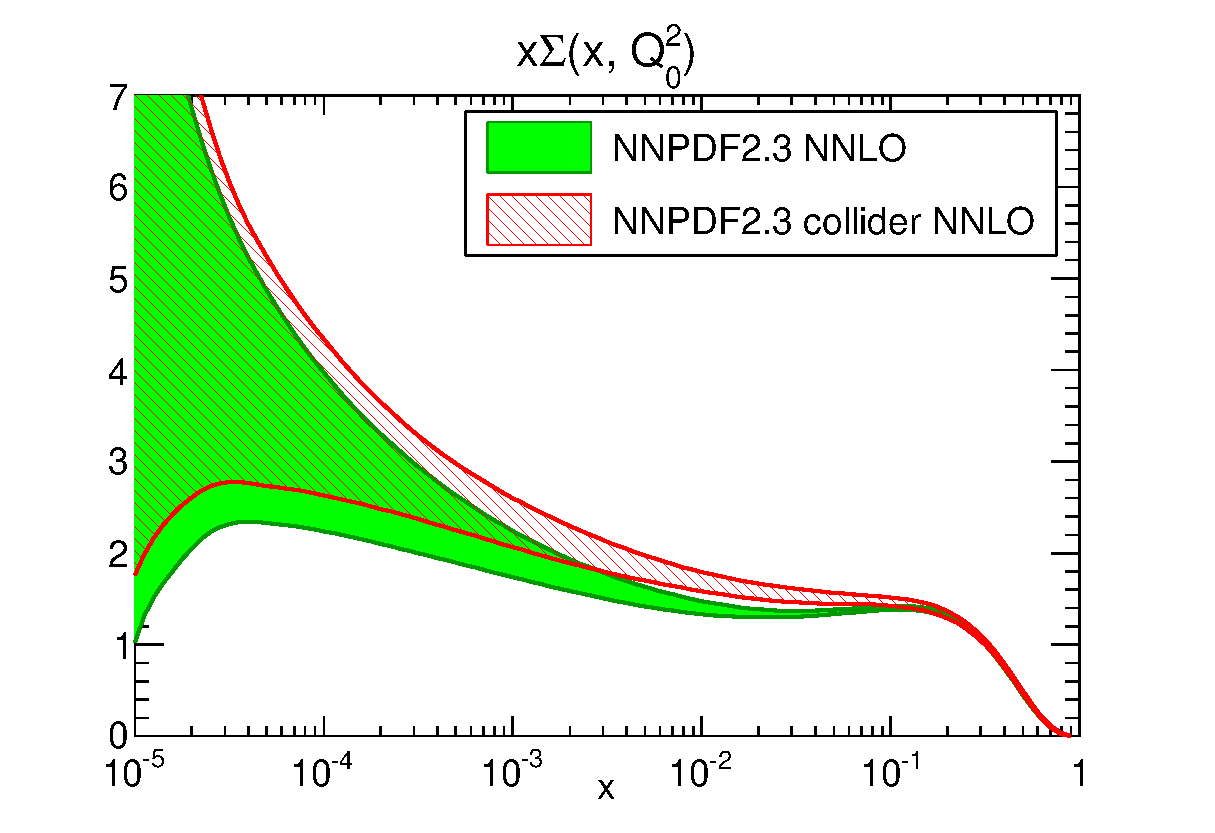
\includegraphics[width=0.5\textwidth]{xSinglet_Q_2_log-23-vs-23coll-nnlo.eps}\\
    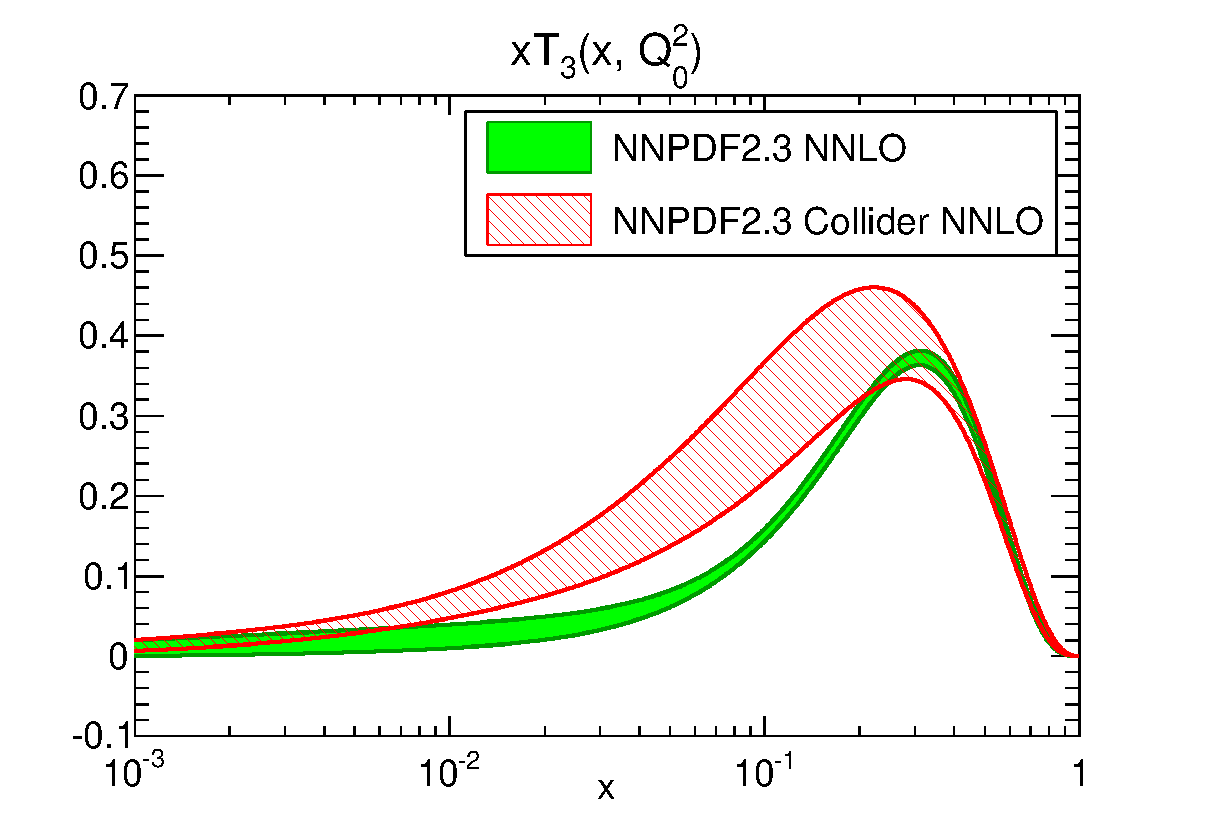
\includegraphics[width=0.5\textwidth]{xT3_Q_2_log-23-vs-23coll-nnlo.eps}
 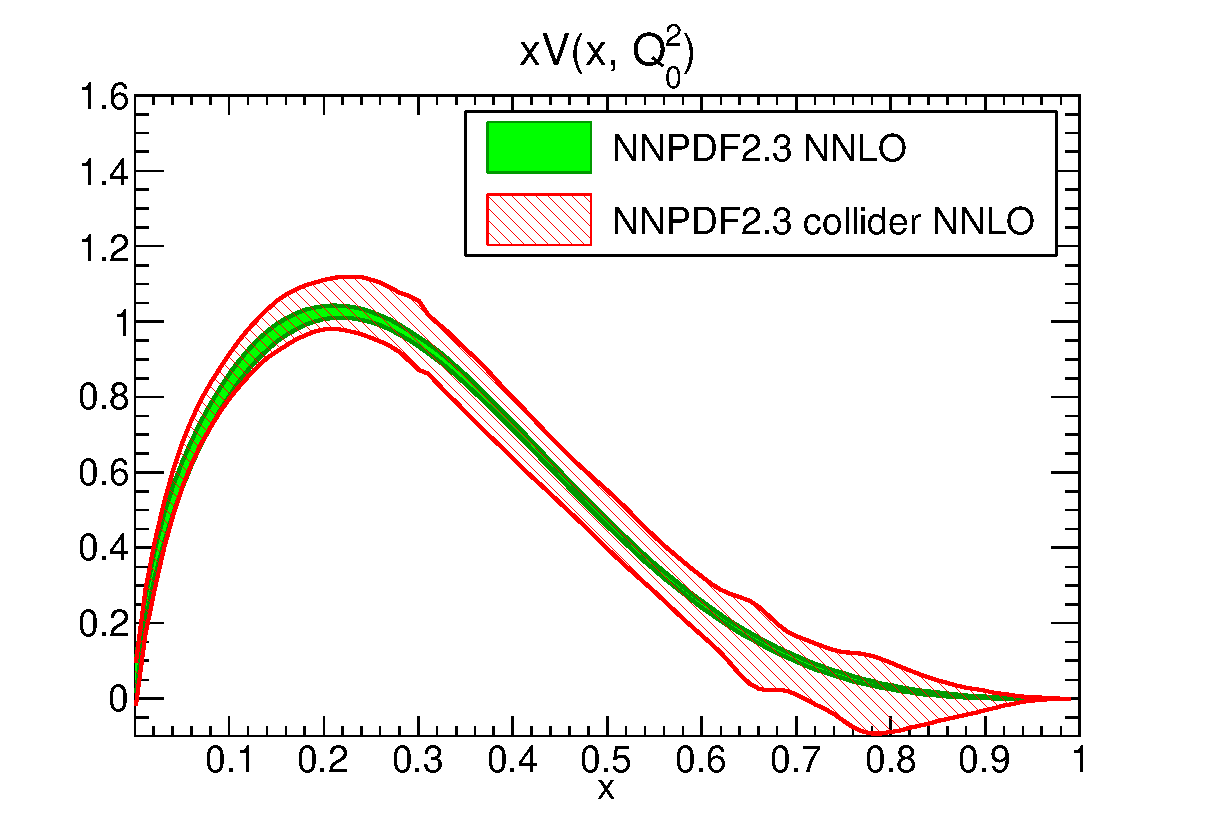
\includegraphics[width=0.5\textwidth]{xV_Q_2_lin-23-vs-23coll-nnlo.eps}
 \end{frame}

%
% \begin{frame}
% \frametitle{MSTW08 Closure test fit}
% \textbf{NNPDF Preliminary}
%    \includegraphics[width=0.5\textwidth]{mstwclosure_singlet.eps}
%   \includegraphics[width=0.5\textwidth]{mstwclosure_gluon.eps}
%   \vskip10pt
%   \begin{itemize}
%   \item<1-> Fit to a generating function determined by a different methodology (MSTW08nlo).
%   \vskip5pt
%   \item<1-> Closure test fit reproduces the generating function within uncertainties.
%   \end{itemize}
% \end{frame}


\begin{frame}
\frametitle{Impact of HT upon NNPDFs}
  \begin{center}    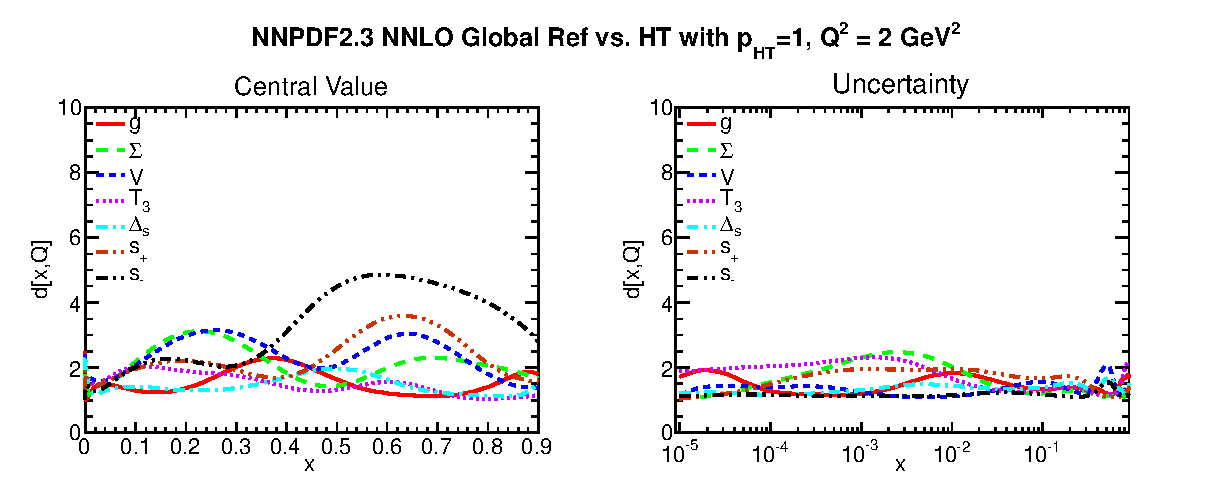
\includegraphics[width=0.8\textwidth]{distances-nnpdf23-global-ref-vs-htp1-2gev2.eps} \\
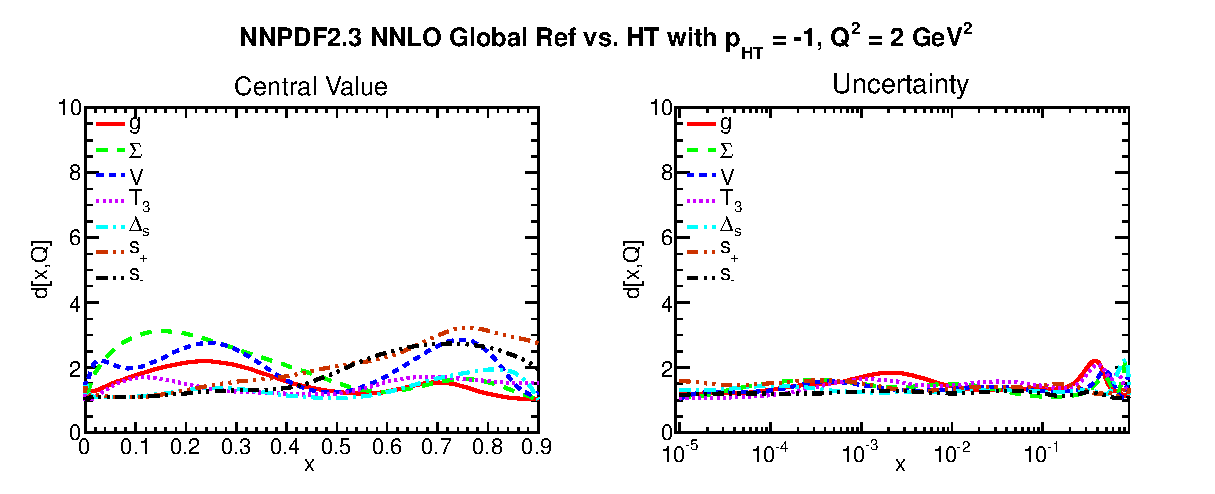
\includegraphics[width=0.8\textwidth]{distances-nnpdf23-global-ref-vs-htm1-2gev2.eps} \end{center}
\end{frame}

\begin{frame}
\frametitle{Impact of deuterium corrections upon NNPDFs}

 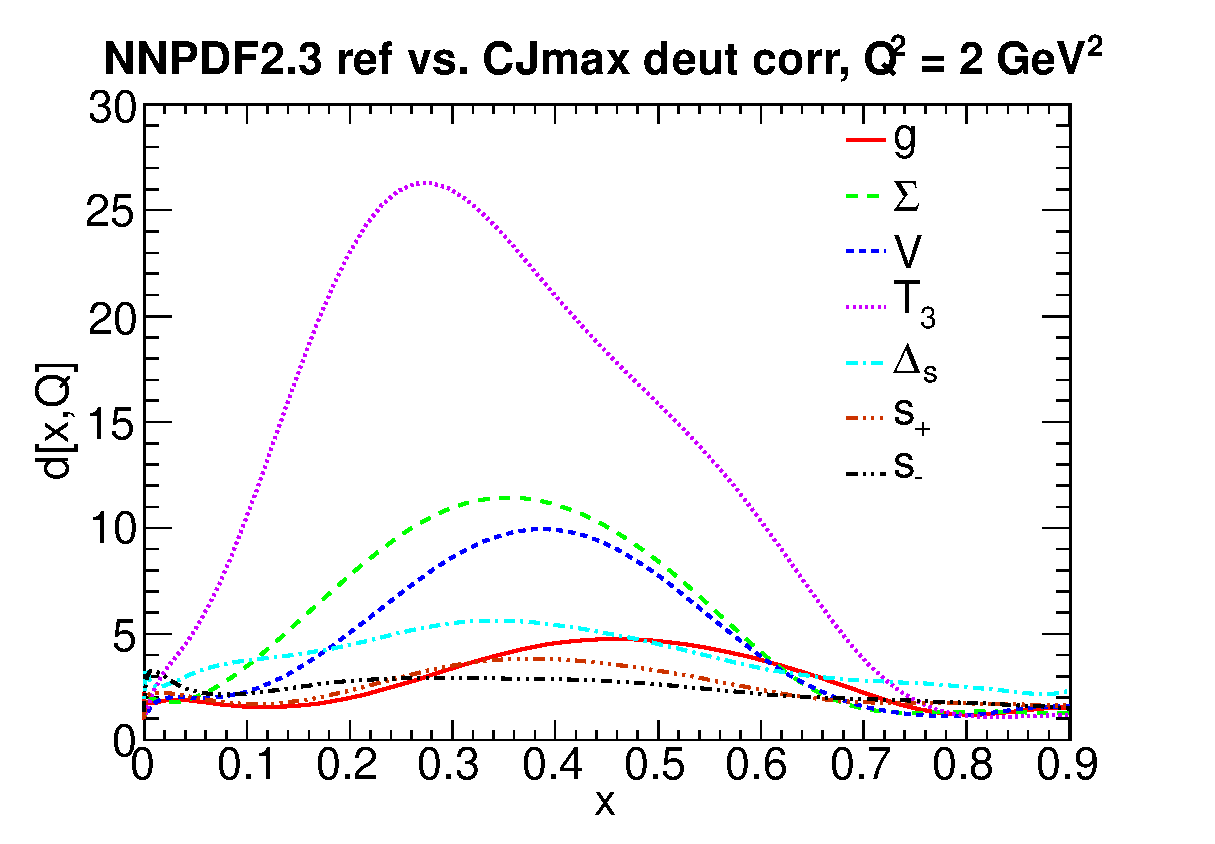
\includegraphics[width=0.5\textwidth]{distances-nnpdf23-deut-cjmax.eps}
 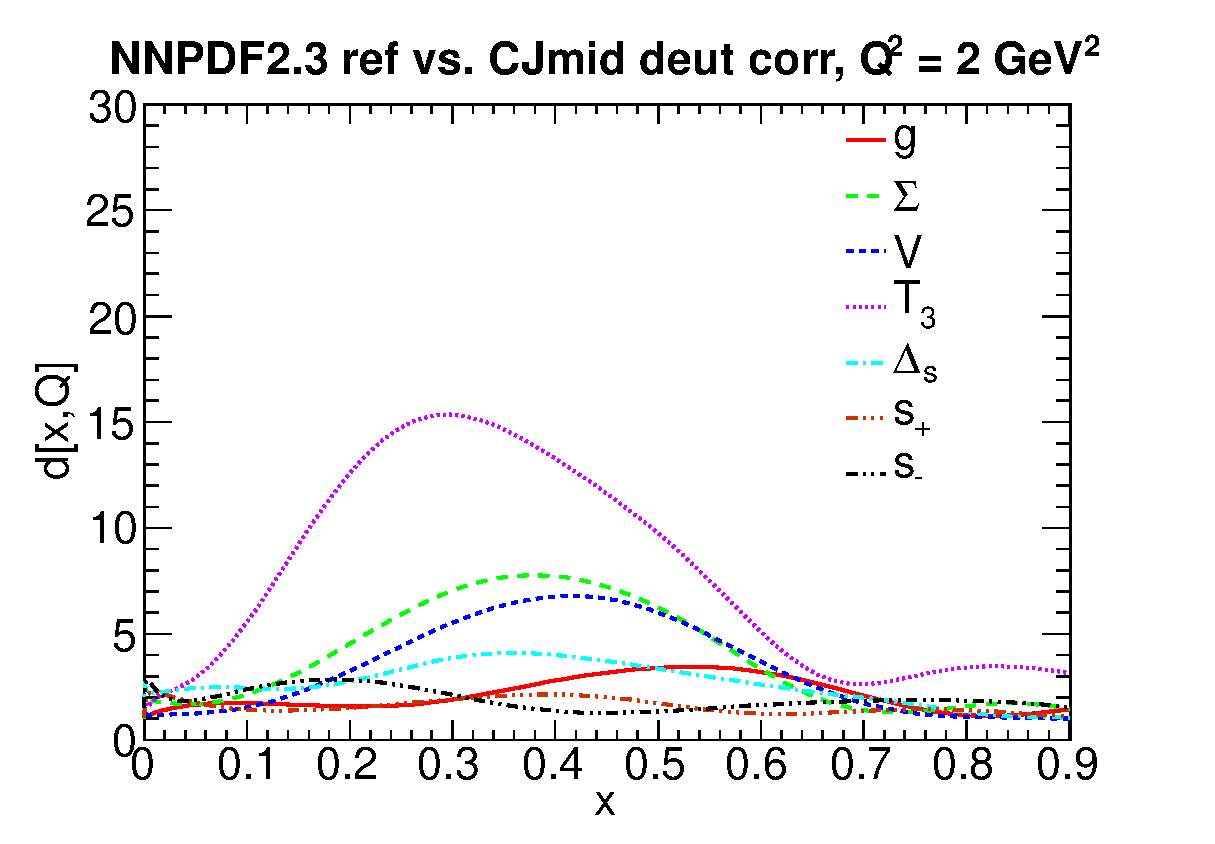
\includegraphics[width=0.5\textwidth]{distances-nnpdf23-deut-cjmid.eps}\\
 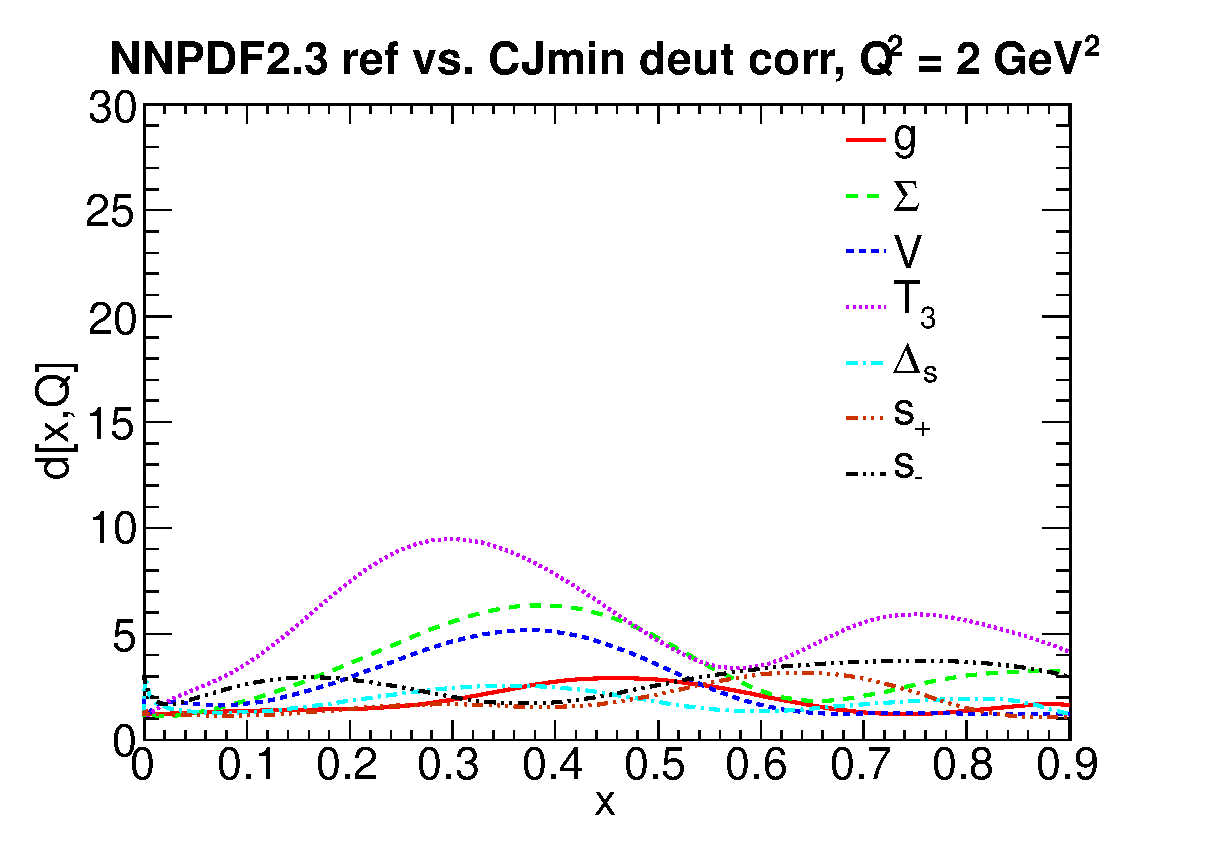
\includegraphics[width=0.5\textwidth]{distances-nnpdf23-deut-cjmin.eps}
 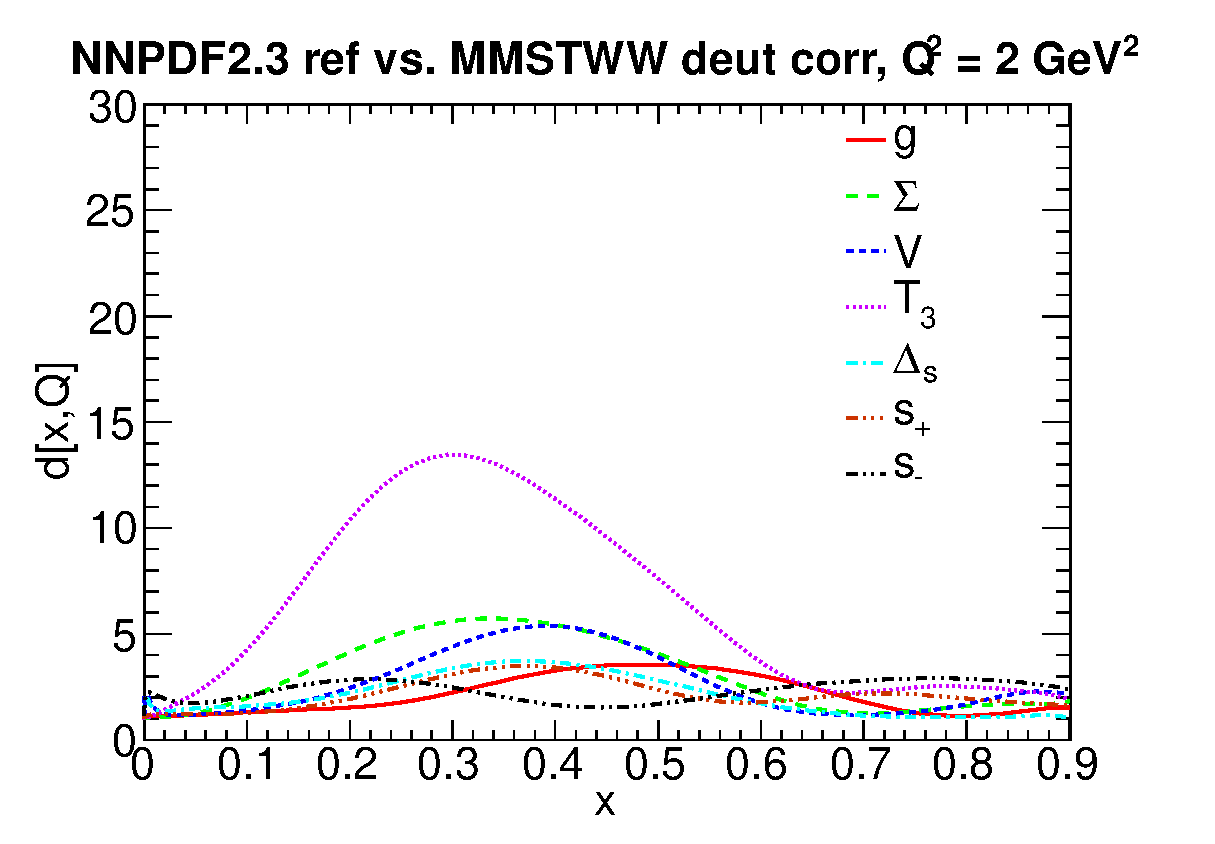
\includegraphics[width=0.5\textwidth]{distances-nnpdf23-deut-mmstww.eps}
\end{frame}

\begin{frame}
\frametitle{Impact of FFN Scheme}
\begin{center} 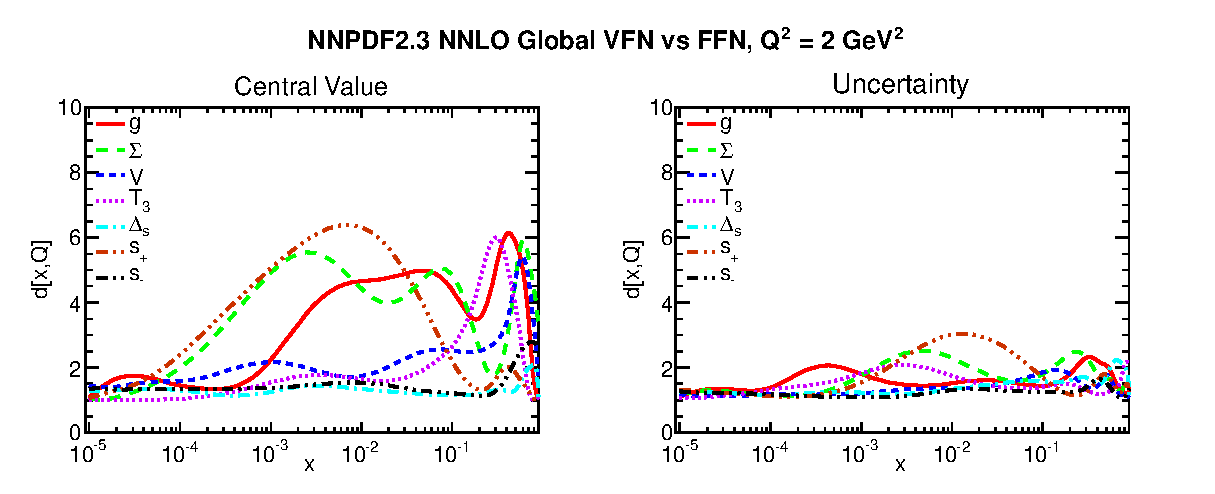
\includegraphics[width=0.8\textwidth]{distances-nnpdf23-global-vfn-vs-ffn-q2-2gev2.eps} \end{center}
\begin{center}   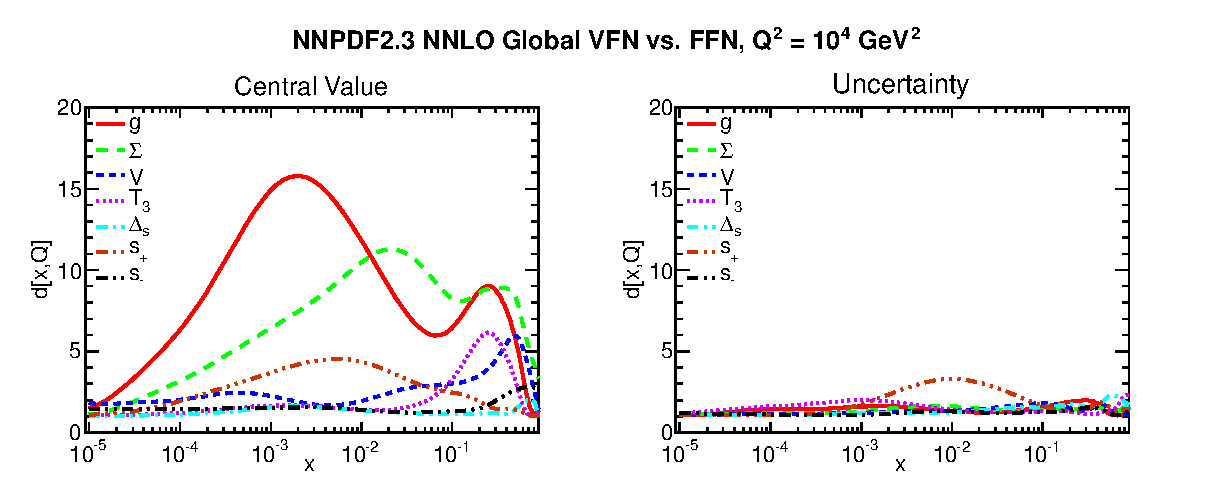
\includegraphics[width=0.8\textwidth]{distances-nnpdf23-global-vfn-vs-ffn-q2-10000gev2.eps} \end{center}
\vskip10pt
\end{frame}


%
%
%
%\begin{frame}
%\small
%\frametitle{Special features of NNPDF approach}
%\textbf{Minimisation by genetic algorithms}\\
%\underline{Problem}: Very large parameter space, $\chi2$ highly nonlocal. \begin{itemize}
%\item<1-> Minimisation is challenging.
%\end{itemize}\underline{Solution}: Genetic Algorithms (GA)
%\begin{itemize}
%\item<1-> Generate mutations of fit parameters.
%\item<1-> Select those mutations that minimise figure of merit.
%\end{itemize}
%\vskip10pt
%\textbf{ Dynamical fit stopping by cross-validation}\\
%\underline{Problem}:  extremely flexible parameterisations are prone to \emph{overfitting}.
%\\
%\begin{itemize}
%\item<1->Fit has so many parameters, the minimum $\chi^2$ corresponds to a fit not only to
%the data, but also statistical noise.
%\end{itemize}
%\underline{Solution}:  dynamical stopping by \emph{Cross Validation}.
%\begin{itemize}
%\item<1-> Split the dataset into a training set and a validation set.
%\item<1-> Use the training set for minimisation, monitor the $\chi^2$ to the validation set.
%\item<1-> Stop the fit when the $\chi^2$ to the validation set starts to increase while
%the $\chi^2$ to training set is still decreasing.
%
%\end{itemize}
%
%
%
%\end{frame}
%
%\begin{frame}
%\frametitle{Cross Validation}
% \begin{figure}[b!]
%    \begin{center}
%      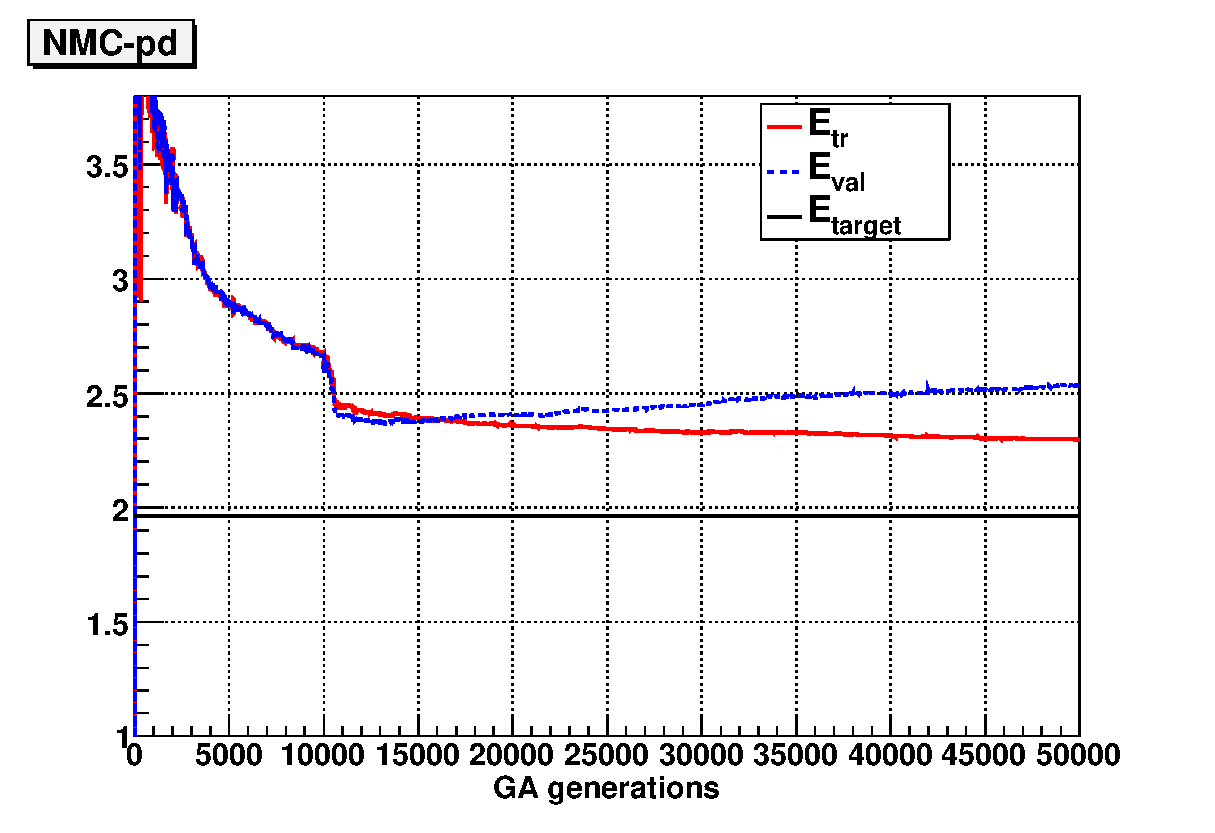
\includegraphics[width=0.9\textwidth]{chi2ite-1004-NMC-pd.eps}
%    \end{center}
%\end{figure}
%\end{frame}
%
%\begin{frame}
%\frametitle{Unweighting procedure}
%\begin{columns}
%  \begin{column}{0.5\textwidth}
%\begin{figure}
%  \epsfig{width=0.7\textwidth,figure=unwplot-1.eps,angle=-90}\\
%\end{figure}
%  \end{column}
%  \begin{column}{0.5\textwidth}
%\begin{figure}
%  \epsfig{width=0.7\textwidth,figure=unwplot-2.eps,angle=-90}
%\end{figure}
%  \end{column}
%\end{columns}
%\end{frame}
%

% End of slides
\end{document}
